% Options for packages loaded elsewhere
\PassOptionsToPackage{unicode}{hyperref}
\PassOptionsToPackage{hyphens}{url}
\PassOptionsToPackage{dvipsnames,svgnames,x11names}{xcolor}
%
\documentclass[
  12pt,
]{extreport}

\usepackage{amsmath,amssymb}
\usepackage{iftex}
\ifPDFTeX
  \usepackage[T1]{fontenc}
  \usepackage[utf8]{inputenc}
  \usepackage{textcomp} % provide euro and other symbols
\else % if luatex or xetex
  \usepackage{unicode-math}
  \defaultfontfeatures{Scale=MatchLowercase}
  \defaultfontfeatures[\rmfamily]{Ligatures=TeX,Scale=1}
\fi
\usepackage{lmodern}
\ifPDFTeX\else  
    % xetex/luatex font selection
\fi
% Use upquote if available, for straight quotes in verbatim environments
\IfFileExists{upquote.sty}{\usepackage{upquote}}{}
\IfFileExists{microtype.sty}{% use microtype if available
  \usepackage[]{microtype}
  \UseMicrotypeSet[protrusion]{basicmath} % disable protrusion for tt fonts
}{}
\makeatletter
\@ifundefined{KOMAClassName}{% if non-KOMA class
  \IfFileExists{parskip.sty}{%
    \usepackage{parskip}
  }{% else
    \setlength{\parindent}{0pt}
    \setlength{\parskip}{6pt plus 2pt minus 1pt}}
}{% if KOMA class
  \KOMAoptions{parskip=half}}
\makeatother
\usepackage{xcolor}
\setlength{\emergencystretch}{3em} % prevent overfull lines
\setcounter{secnumdepth}{-\maxdimen} % remove section numbering
% Make \paragraph and \subparagraph free-standing
\makeatletter
\ifx\paragraph\undefined\else
  \let\oldparagraph\paragraph
  \renewcommand{\paragraph}{
    \@ifstar
      \xxxParagraphStar
      \xxxParagraphNoStar
  }
  \newcommand{\xxxParagraphStar}[1]{\oldparagraph*{#1}\mbox{}}
  \newcommand{\xxxParagraphNoStar}[1]{\oldparagraph{#1}\mbox{}}
\fi
\ifx\subparagraph\undefined\else
  \let\oldsubparagraph\subparagraph
  \renewcommand{\subparagraph}{
    \@ifstar
      \xxxSubParagraphStar
      \xxxSubParagraphNoStar
  }
  \newcommand{\xxxSubParagraphStar}[1]{\oldsubparagraph*{#1}\mbox{}}
  \newcommand{\xxxSubParagraphNoStar}[1]{\oldsubparagraph{#1}\mbox{}}
\fi
\makeatother

\usepackage{color}
\usepackage{fancyvrb}
\newcommand{\VerbBar}{|}
\newcommand{\VERB}{\Verb[commandchars=\\\{\}]}
\DefineVerbatimEnvironment{Highlighting}{Verbatim}{commandchars=\\\{\}}
% Add ',fontsize=\small' for more characters per line
\usepackage{framed}
\definecolor{shadecolor}{RGB}{241,243,245}
\newenvironment{Shaded}{\begin{snugshade}}{\end{snugshade}}
\newcommand{\AlertTok}[1]{\textcolor[rgb]{0.68,0.00,0.00}{#1}}
\newcommand{\AnnotationTok}[1]{\textcolor[rgb]{0.37,0.37,0.37}{#1}}
\newcommand{\AttributeTok}[1]{\textcolor[rgb]{0.40,0.45,0.13}{#1}}
\newcommand{\BaseNTok}[1]{\textcolor[rgb]{0.68,0.00,0.00}{#1}}
\newcommand{\BuiltInTok}[1]{\textcolor[rgb]{0.00,0.23,0.31}{#1}}
\newcommand{\CharTok}[1]{\textcolor[rgb]{0.13,0.47,0.30}{#1}}
\newcommand{\CommentTok}[1]{\textcolor[rgb]{0.37,0.37,0.37}{#1}}
\newcommand{\CommentVarTok}[1]{\textcolor[rgb]{0.37,0.37,0.37}{\textit{#1}}}
\newcommand{\ConstantTok}[1]{\textcolor[rgb]{0.56,0.35,0.01}{#1}}
\newcommand{\ControlFlowTok}[1]{\textcolor[rgb]{0.00,0.23,0.31}{\textbf{#1}}}
\newcommand{\DataTypeTok}[1]{\textcolor[rgb]{0.68,0.00,0.00}{#1}}
\newcommand{\DecValTok}[1]{\textcolor[rgb]{0.68,0.00,0.00}{#1}}
\newcommand{\DocumentationTok}[1]{\textcolor[rgb]{0.37,0.37,0.37}{\textit{#1}}}
\newcommand{\ErrorTok}[1]{\textcolor[rgb]{0.68,0.00,0.00}{#1}}
\newcommand{\ExtensionTok}[1]{\textcolor[rgb]{0.00,0.23,0.31}{#1}}
\newcommand{\FloatTok}[1]{\textcolor[rgb]{0.68,0.00,0.00}{#1}}
\newcommand{\FunctionTok}[1]{\textcolor[rgb]{0.28,0.35,0.67}{#1}}
\newcommand{\ImportTok}[1]{\textcolor[rgb]{0.00,0.46,0.62}{#1}}
\newcommand{\InformationTok}[1]{\textcolor[rgb]{0.37,0.37,0.37}{#1}}
\newcommand{\KeywordTok}[1]{\textcolor[rgb]{0.00,0.23,0.31}{\textbf{#1}}}
\newcommand{\NormalTok}[1]{\textcolor[rgb]{0.00,0.23,0.31}{#1}}
\newcommand{\OperatorTok}[1]{\textcolor[rgb]{0.37,0.37,0.37}{#1}}
\newcommand{\OtherTok}[1]{\textcolor[rgb]{0.00,0.23,0.31}{#1}}
\newcommand{\PreprocessorTok}[1]{\textcolor[rgb]{0.68,0.00,0.00}{#1}}
\newcommand{\RegionMarkerTok}[1]{\textcolor[rgb]{0.00,0.23,0.31}{#1}}
\newcommand{\SpecialCharTok}[1]{\textcolor[rgb]{0.37,0.37,0.37}{#1}}
\newcommand{\SpecialStringTok}[1]{\textcolor[rgb]{0.13,0.47,0.30}{#1}}
\newcommand{\StringTok}[1]{\textcolor[rgb]{0.13,0.47,0.30}{#1}}
\newcommand{\VariableTok}[1]{\textcolor[rgb]{0.07,0.07,0.07}{#1}}
\newcommand{\VerbatimStringTok}[1]{\textcolor[rgb]{0.13,0.47,0.30}{#1}}
\newcommand{\WarningTok}[1]{\textcolor[rgb]{0.37,0.37,0.37}{\textit{#1}}}

\providecommand{\tightlist}{%
  \setlength{\itemsep}{0pt}\setlength{\parskip}{0pt}}\usepackage{longtable,booktabs,array}
\usepackage{calc} % for calculating minipage widths
% Correct order of tables after \paragraph or \subparagraph
\usepackage{etoolbox}
\makeatletter
\patchcmd\longtable{\par}{\if@noskipsec\mbox{}\fi\par}{}{}
\makeatother
% Allow footnotes in longtable head/foot
\IfFileExists{footnotehyper.sty}{\usepackage{footnotehyper}}{\usepackage{footnote}}
\makesavenoteenv{longtable}
\usepackage{graphicx}
\makeatletter
\def\maxwidth{\ifdim\Gin@nat@width>\linewidth\linewidth\else\Gin@nat@width\fi}
\def\maxheight{\ifdim\Gin@nat@height>\textheight\textheight\else\Gin@nat@height\fi}
\makeatother
% Scale images if necessary, so that they will not overflow the page
% margins by default, and it is still possible to overwrite the defaults
% using explicit options in \includegraphics[width, height, ...]{}
\setkeys{Gin}{width=\maxwidth,height=\maxheight,keepaspectratio}
% Set default figure placement to htbp
\makeatletter
\def\fps@figure{htbp}
\makeatother

\usepackage{booktabs}
\usepackage{longtable}
\usepackage{array}
\usepackage{multirow}
\usepackage{wrapfig}
\usepackage{float}
\usepackage{colortbl}
\usepackage{pdflscape}
\usepackage{tabu}
\usepackage{threeparttable}
\usepackage{threeparttablex}
\usepackage[normalem]{ulem}
\usepackage{makecell}
\usepackage{xcolor}
\usepackage[a4paper, margin=1.2in]{geometry}
\usepackage{graphicx}
\usepackage{float}
\usepackage{anyfontsize}
\usepackage{titling}
\pretitle{\begin{center}\Huge\bfseries}
\posttitle{\par\end{center}}
\preauthor{\begin{center}\large}
\postauthor{\par\end{center}}
\predate{\begin{center}\large}
\postdate{\par\end{center}}
\usepackage{fancyhdr}
\pagestyle{fancy}
\fancyhead{}
\fancyhead[L]{Jorge Ruiz López}
\fancyhead[R]{\leftmark}
\fancyfoot[C]{\thepage}
\makeatletter
\@ifpackageloaded{caption}{}{\usepackage{caption}}
\AtBeginDocument{%
\ifdefined\contentsname
  \renewcommand*\contentsname{Table of contents}
\else
  \newcommand\contentsname{Table of contents}
\fi
\ifdefined\listfigurename
  \renewcommand*\listfigurename{List of Figures}
\else
  \newcommand\listfigurename{List of Figures}
\fi
\ifdefined\listtablename
  \renewcommand*\listtablename{List of Tables}
\else
  \newcommand\listtablename{List of Tables}
\fi
\ifdefined\figurename
  \renewcommand*\figurename{Figure}
\else
  \newcommand\figurename{Figure}
\fi
\ifdefined\tablename
  \renewcommand*\tablename{Table}
\else
  \newcommand\tablename{Table}
\fi
}
\@ifpackageloaded{float}{}{\usepackage{float}}
\floatstyle{ruled}
\@ifundefined{c@chapter}{\newfloat{codelisting}{h}{lop}}{\newfloat{codelisting}{h}{lop}[chapter]}
\floatname{codelisting}{Listing}
\newcommand*\listoflistings{\listof{codelisting}{List of Listings}}
\makeatother
\makeatletter
\makeatother
\makeatletter
\@ifpackageloaded{caption}{}{\usepackage{caption}}
\@ifpackageloaded{subcaption}{}{\usepackage{subcaption}}
\makeatother

\ifLuaTeX
  \usepackage{selnolig}  % disable illegal ligatures
\fi
\usepackage{bookmark}

\IfFileExists{xurl.sty}{\usepackage{xurl}}{} % add URL line breaks if available
\urlstyle{same} % disable monospaced font for URLs
\hypersetup{
  pdftitle={Análisis estadístico de la Pokédex nacional},
  pdfauthor={Jorge Ruiz López},
  colorlinks=true,
  linkcolor={blue},
  filecolor={Maroon},
  citecolor={Blue},
  urlcolor={Blue},
  pdfcreator={LaTeX via pandoc}}


\title{Análisis estadístico de la Pokédex nacional}
\author{Jorge Ruiz López}
\date{2025-01-23}

\begin{document}
\maketitle


\maketitle

\chapter{Índice}\label{uxedndice}

\begin{enumerate}
\def\labelenumi{\arabic{enumi}.}
\item
  Introducción y contexto
\item
  Estudio inicial de los datos

  2.1. Lectura, análisis y limpieza del dataset

  2.2. Estudio global de los datos

  2.3. Estudio de los datos por grupos
\item
  Análisis de componentes principales

  3.1. Cálculo de las componentes principales

  3.2. Análisis de las componentes principales
\item
  Análisis cluster

  4.1. Introducción y consideraciones previas

  4.2. Caso práctico

  4.3. Conclusiones
\item
  Regresión Lineal Múltiple
\end{enumerate}

\chapter{1. Introducción y contexto}\label{introducciuxf3n-y-contexto}

En el presente documento, analizaremos exhaustivamente el conjunto de
datos en cuestión es una versión en formato CSV de la base de datos
relacional que contiene los datos de 1025 especies de Pokémon (criaturas
de la franquicia de videojuegos homónima). Aplicaremos sobre él diversas
técnicas de análisis multivariante.

Para cada observación de una especie de Pokémon, nuestro dataset ofrece
información sobre 14 variables. Debido a las distintas naturalezas de
las características observables en un Pokémon, vamos a dividirlas en dos
grupos:

\begin{itemize}
\item
  Características descriptivas - Todas son de tipo \texttt{chr} (cadenas
  de texto) excepto el \texttt{id}:

  \begin{itemize}
  \item
    \texttt{pokemon\_id}: Identificador único para cada Pokémon,
    correspondiente con su número en la Pokédex global (donde se recoge
    la información oficial de todos los Pokémon que existen, y podemos
    encontrarla en el sitio web oficial de la franquicia:
    \href{https://www.pokemon.com/es/pokedex}{\emph{https://www.pokemon.com/es/pokedex}}\emph{)}.
  \item
    \texttt{name}: Nombre oficial de cada Pokémon, único para cada uno.
  \item
    \texttt{primary\_type}: Tipo principal del Pokémon. Todos tienen
    uno, y puede tomar un valor de 18 distintos.
  \item
    \texttt{secondary\_type}: Tipo secundario del Pokémon. No siempre es
    aplicable (hay Pokémon que son puramente de un tipo), y puede tomar
    los mismos valores que el principal.
  \item
    \texttt{first\_appreance}: Juego en el que el Pokémon apareció por
    primera vez (p.e: ``Red/Blue'' refiriéndose a las primeras entregas
    antes comentadas).
  \item
    \texttt{generation}: Generación a la que el Pokémon pertenece, de
    las 9 comentadas anteriormente.
  \item
    \texttt{category}: Categoría del Pokémon (hay 5 posibles de más
    común a más raro: ``regular'', ``legendary'', ``mythical'' o
    singulares, ``ultra beast'' o ``ultraentes'', y ``paradox'' o
    ``paradoja''). La categoría de ultraente sólo está disponible a
    partir de la séptima generación, y la ``paradox'' es exclusiva de la
    última.
  \end{itemize}
\item
  Estadísticas numéricas (\texttt{int}):

  \begin{itemize}
  \item
    \texttt{total\_base\_stats}: Suma de estadísticas del Pokémon. Para
    cada uno, es la suma de las otras 6 variables.
  \item
    \texttt{hp}: ``Hit points'' (puntos de salud), daño que un Pokémon
    puede recibir antes de debilitarse.
  \item
    \texttt{attack}: Puntos de daño que inflinge un ataque básico del
    Pokémon.
  \item
    \texttt{defense}: Defensa básica del Pokémon (resistencia a ataques
    básicos).
  \item
    \texttt{special\_attack}: Puntos de daño que inflinge el Pokémon con
    su ataque especial.
  \item
    \texttt{special\_defense}: Defensa del Pokémon ante ataques
    especiales.
  \item
    \texttt{speed}: Velocidad del Pokémon.
  \end{itemize}
\end{itemize}

\subsubsection{Objetivos:}\label{objetivos}

Merece la pena mencionar que la franquicia de Pokémon se ha expandido
más allá de las consolas de videojuegos. Podemos recordar fenómenos
globales como el célebre ``Pokémon Go''; o el juego de cartas
coleccionables, cuyo mercado mueve una gran cantidad de dinero. El
análisis que realizaremos en base a todas estas estadísticas busca ser
de utilidad para:

\begin{itemize}
\item
  Planificar una buena estrategia en los combates Pokémon. Adquirir
  maestría en ellos depende en gran medida de la estrategia que
  desarrollemos en base a nuestro conocimiento del juego. Demostraremos
  que la estadística es una herramienta poderosísima para obtener buenos
  resultados, aún sin conocimientos previos del campo.
\item
  Decidir qué Pokémon es mejor atrapar o conseguir para formar nuestro
  equipo.
\item
  Fines lúdicos, de forma que los fans de la franquicia puedan disfrutar
  el análisis y quizás ampliar su conocimiento del universo Pokémon.
\end{itemize}

\subsubsection{Fuentes:}\label{fuentes}

El dataset ha sido obtenido de la plataforma ``Kaggle'', ampliamente
conocida entre los científicos de datos y profesionales del Machine
Learning. Se puede acceder a él desde este enlace:
\href{https://www.kaggle.com/datasets/pauloarayasantiago/pokmon-stats-across-generations-and-typings}{\emph{https://www.kaggle.com/datasets/pauloarayasantiago/pokmon-stats-across-generations-and-typings}}.

Investigando un poco sobre de dónde se han obtenido estos datos para
presentarlos de forma más organizada en el CSV, vemos que vienen de la
API (interfaz de programación de aplicaciones) de tipo REST ``PokéAPI''
(\href{https://pokeapi.co/}{\emph{https://pokeapi.co/}}). En ella,
podemos encontrar todos los datos oficiales de la franquicia, con
información completamente actualizada, a través de distintos tipos de
consultas.

\chapter{2. Estudio inicial de los
datos}\label{estudio-inicial-de-los-datos}

\section{2.1. Lectura, análisis y limpieza del
dataset}\label{lectura-anuxe1lisis-y-limpieza-del-dataset}

Comenzamos leyendo el fichero de datos y observando que el formato
coincide con el descrito:

\begin{verbatim}
'data.frame':   1025 obs. of  14 variables:
 $ pokemon_id      : int  1 2 3 4 5 6 7 8 9 10 ...
 $ name            : chr  "bulbasaur" "ivysaur" "venusaur" "charmander" ...
 $ primary_type    : chr  "grass" "grass" "grass" "fire" ...
 $ secondary_type  : chr  "poison" "poison" "poison" "" ...
 $ first_appreance : chr  "red/blue" "red/blue" "red/blue" "red/blue" ...
 $ generation      : chr  "gen 1" "gen 1" "gen 1" "gen 1" ...
 $ category        : chr  "regular" "regular" "regular" "regular" ...
 $ total_base_stats: int  318 405 525 309 405 534 314 405 530 195 ...
 $ hp              : int  45 60 80 39 58 78 44 59 79 45 ...
 $ attack          : int  49 62 82 52 64 84 48 63 83 30 ...
 $ defense         : int  49 63 83 43 58 78 65 80 100 35 ...
 $ special_attack  : int  65 80 100 60 80 109 50 65 85 20 ...
 $ special_defense : int  65 80 100 50 65 85 64 80 105 20 ...
 $ speed           : int  45 60 80 65 80 100 43 58 78 45 ...
\end{verbatim}

Vemos que el primer Pokémon en la Pokédex es Bulbasaur, de tipo planta y
veneno, de la primera generación, y con una suma de estadísticas de 318
puntos. Antes de nada, vamos a limpiar el dataset para considerar 11
variables en vez de 14. Eliminaremos las variables: \texttt{pokemon\_id}
(inferible a partir del índice del Pokémon en el dataframe),
\texttt{secondary\_type} (nos centraremos en un sólo tipo), y
\texttt{first\_appreance} (no aporta información relevante al estudio).

Además del nombre, que sabemos que es único para cada Pokémon, nos
interesa saber cuántos valores posibles toman el resto de variables de
tipo \texttt{chr}.

Tipos:

\begin{verbatim}
 [1] "grass"    "fire"     "water"    "bug"      "normal"   "poison"  
 [7] "electric" "ground"   "fairy"    "fighting" "psychic"  "rock"    
[13] "ghost"    "ice"      "dragon"   "dark"     "steel"    "flying"  
\end{verbatim}

Generaciones:

\begin{verbatim}
[1] "gen 1" "gen 2" "gen 3" "gen 4" "gen 5" "gen 6" "gen 7" "gen 8" "gen 9"
\end{verbatim}

Categorías:

\begin{verbatim}
[1] "regular"     "legendary"   "mythical"    "ultra beast" "paradox"    
\end{verbatim}

Vemos ya desde el principio que hay 3 variables que pueden ser
categóricas, y nos pueden servir para realizar estudios agrupando los
Pokémon por tipo, generación o categoría.

\section{2.2. Estudio global de los
datos}\label{estudio-global-de-los-datos}

Antes de agrupar, vamos a resumir las principales características de
nuestro dataset de forma global, considerando por igual todas las
observaciones. Nos centraremos en las variables numéricas, pudiendo dar
el valor de las principales medidas descriptivas (daremos el rango
\((min, max)\) y la media).

\begin{table}[H]
\centering
\begin{tabular}{lrrr}
\toprule
  & media & min & max\\
\midrule
total\_base\_stats & 427.68683 & 175 & 720\\
hp & 70.18439 & 1 & 255\\
attack & 77.52195 & 5 & 181\\
defense & 72.50732 & 5 & 230\\
special\_attack & 70.08098 & 10 & 173\\
\addlinespace
special\_defense & 70.20585 & 20 & 230\\
speed & 67.18634 & 5 & 200\\
\bottomrule
\end{tabular}
\end{table}

Podemos ver que las escalas son similares, excepto la de la variable
total\_base\_stats (``total'' a partir de ahora para abreviar), lo cual
tiene sentido ya que esta es la suma de las otras 6 en cada fila. Los
valores medios de todas las variables (excepto ``total'') son cercanos
(entre 65 y 75). No obstante, podemos ver que las 7 variables toman
valores en rangos muy amplios.

Calculamos también la matriz de covarianzas muestrales:

\begin{table}[H]
\centering\begingroup\fontsize{9}{11}\selectfont

\begin{tabular}{rrrrrrr}
\toprule
12717.239 & 2003.5168 & 2399.3687 & 2078.944188 & 2345.0771 & 2096.8819 & 1793.450015\\
2003.517 & 709.2130 & 377.6468 & 233.213005 & 284.0368 & 261.8429 & 137.564240\\
2399.369 & 377.6468 & 886.9998 & 406.084556 & 248.9850 & 179.4051 & 300.247370\\
2078.944 & 233.2130 & 406.0846 & 857.726753 & 182.4999 & 392.6523 & 6.767678\\
2345.077 & 284.0368 & 248.9850 & 182.499895 & 879.6194 & 389.5360 & 360.399935\\
\addlinespace
2096.882 & 261.8429 & 179.4051 & 392.652301 & 389.5360 & 709.6539 & 163.791682\\
1793.450 & 137.5642 & 300.2474 & 6.767678 & 360.3999 & 163.7917 & 824.679110\\
\bottomrule
\end{tabular}
\endgroup{}
\end{table}

Y la matriz de correlaciones:

\begin{table}[H]
\centering\begingroup\fontsize{9}{11}\selectfont

\begin{tabular}{rrrrrrr}
\toprule
1.0000000 & 0.6671265 & 0.7143957 & 0.6294655 & 0.7011538 & 0.6979982 & 0.5537967\\
0.6671265 & 1.0000000 & 0.4761412 & 0.2990129 & 0.3596159 & 0.3690873 & 0.1798766\\
0.7143957 & 0.4761412 & 1.0000000 & 0.4655649 & 0.2818799 & 0.2261257 & 0.3510548\\
0.6294655 & 0.2990129 & 0.4655649 & 1.0000000 & 0.2101071 & 0.5032808 & 0.0080468\\
0.7011538 & 0.3596159 & 0.2818799 & 0.2101071 & 1.0000000 & 0.4930341 & 0.4231504\\
\addlinespace
0.6979982 & 0.3690873 & 0.2261257 & 0.5032808 & 0.4930341 & 1.0000000 & 0.2141046\\
0.5537967 & 0.1798766 & 0.3510548 & 0.0080468 & 0.4231504 & 0.2141046 & 1.0000000\\
\bottomrule
\end{tabular}
\endgroup{}
\end{table}

Se aprecia que las escalas (varianzas) son, en general, similares,
exceptuando la variable ``total''. La matriz de correlaciones puede ir
acompañada del gráfico de correlaciones. Empleando ambos, podremos dar
información sobre las relaciones de dependencia entre las variables.

\begin{center}
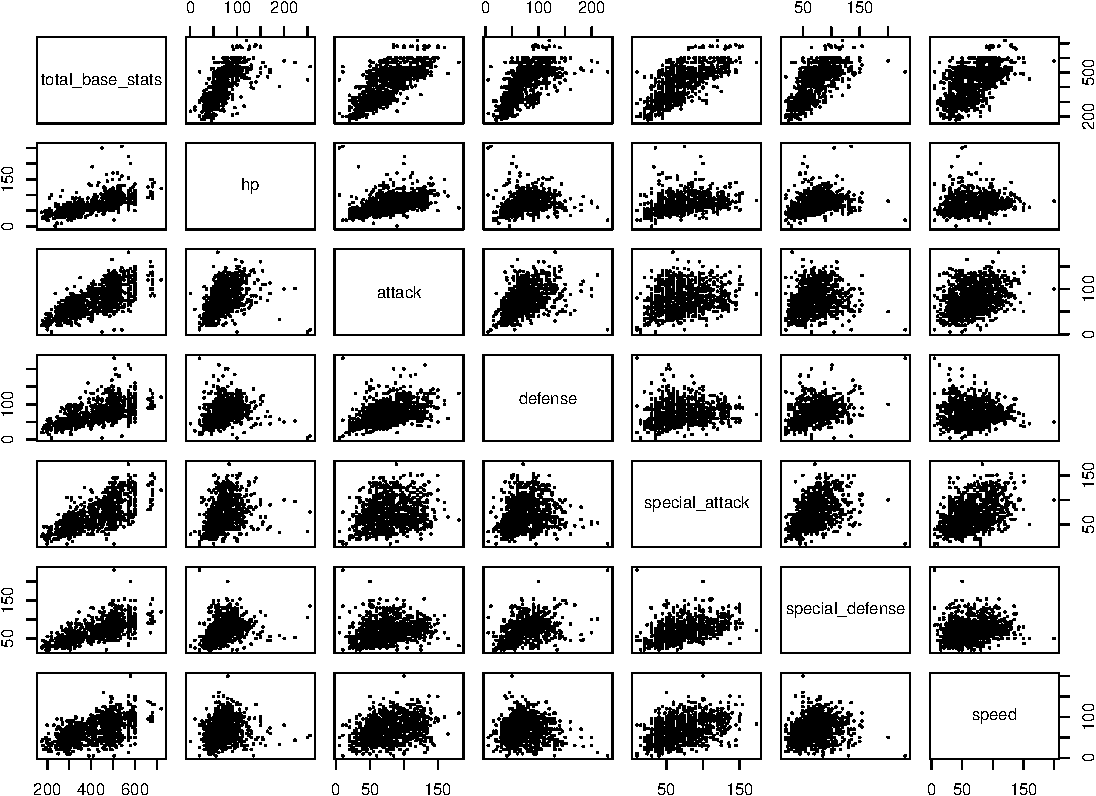
\includegraphics{trabajo_files/figure-pdf/unnamed-chunk-10-1.pdf}
\end{center}

Observamos que todas las variables, en caso de relacionarse, lo hacen de
forma positiva. Esto viene sustentado también por la matriz de
correlaciones de arriba (todas las entradas positivas). También hay
algunas variables incorreladas o con muy poca correlación.

Encontramos las correlaciones más fuertes entre todas las variables a
partir de hp (exceptuando quizás speed) con la variable ``total''.
Podemos ver que la tendencia en estas gráficas es la más creciente y los
puntos están más condensados que en el resto. Esto tiene sentido, ya que
``total'' es una variable calculada a partir de la suma de las otras 6,
por lo que es de esperar que su dependencia de ellas sea media/alta.
Destaca la correlación casi nula entre las variables defense y speed,
pudiendo considerarse incorreladas.

Parece haber varios atípicos respecto a la normal en todos
(observaciones que no siguen el comportamiento esperado según lo que es
habitual). Aunque a simple vista no parece que haber diferencias claras
de grupos, quizás podríamos trazar una separación entre un grupo
mayoritario, y una minoría que queda por arriba en algunas variables
(apartado 2.3).

Podemos hacer también los diagramas de caja-bigotes. Como ``total'' toma
valores más altos que las demás al ser la suma, la hacemos por separado
(su escala es muy distinta de las demás).

\begin{figure}

\begin{minipage}{0.50\linewidth}
\begin{center}
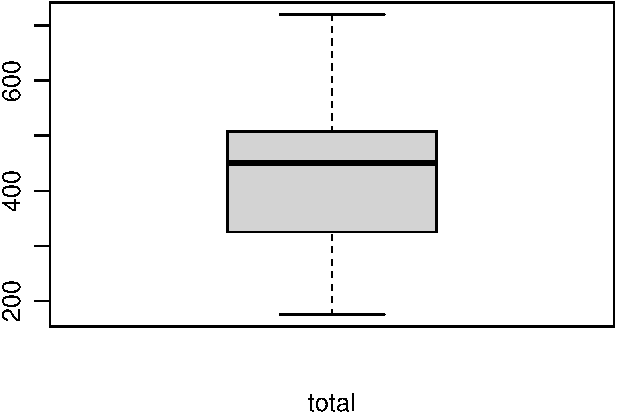
\includegraphics{trabajo_files/figure-pdf/unnamed-chunk-11-1.pdf}
\end{center}
\end{minipage}%
%
\begin{minipage}{0.50\linewidth}
\begin{center}
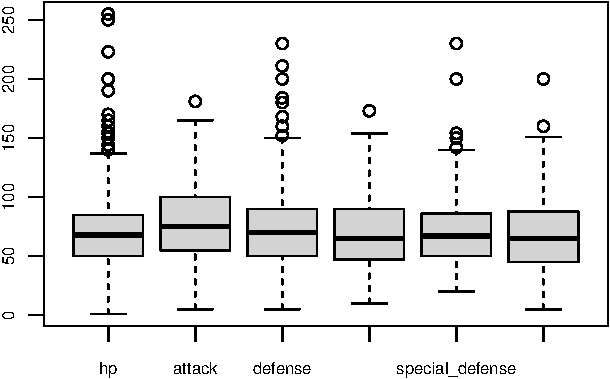
\includegraphics{trabajo_files/figure-pdf/unnamed-chunk-11-2.pdf}
\end{center}
\end{minipage}%

\end{figure}%

En el de la derecha, las variables están en el siguiente orden: hp,
attack, defense, special\_attack, special\_defense, speed (se podría
poner más grande para que se vieran todas, pero hay algunas con nombre
muy largo y nos saldrían gráficas demasiado grandes). Percibimos varios
atípicos respecto de la normal, que se consideran raros ``por arriba''.
El hecho de que no haya atípicos en ``total'' (según el diagrama de
caja) tiene sentido, ya que estamos hablando de criaturas de un
videojuego. Para que funcione, este debe estar balanceado. Un atípico en
``total'' evidenciaría la existencia de un Pokémon notablemente mejor o
peor que todos los demás (rompería el juego). Además, vemos que la
escala de ``total'' es muy diferente a la del resto de variables, que
son similares en cuanto a escala (como habíamos dicho observando las
varianzas).

Vemos que el equilibrio global suele conseguirse ya que los Pokémon que
destacan por tener un atributo demasiado alto, suelen estar compensados
teniendo el resto más bajos. Por ejemplo, si estudiamos cuál es el
Pokémon con mayor hp, es decir, el atípico de más arriba en el
correspondiente diagrama:

\begin{table}[H]
\centering\begingroup\fontsize{9.5}{11.5}\selectfont

\begin{tabular}{llrrrrrrr}
\toprule
  & name & total\_base\_stats & hp & attack & defense & special\_attack & special\_defense & speed\\
\midrule
242 & blissey & 540 & 255 & 10 & 10 & 75 & 135 & 55\\
\bottomrule
\end{tabular}
\endgroup{}
\end{table}

Se trata de Blissey. Este Pokémon no destaca en ``total'' (está
ligeramente por encima de la media); y detectamos que su ataque y
defensa son nefastos, 5 puntos por encima del mínimo. Viendo el Pokémon
que es atípico para la variable attack:

\begin{table}[H]
\centering\begingroup\fontsize{9.5}{11.5}\selectfont

\begin{tabular}{llrrrrrrr}
\toprule
  & name & total\_base\_stats & hp & attack & defense & special\_attack & special\_defense & speed\\
\midrule
798 & kartana & 570 & 59 & 181 & 131 & 59 & 31 & 109\\
\bottomrule
\end{tabular}
\endgroup{}
\end{table}

Es Kartana, que tiene un ataque excepcional, una defensa buena, pero un
hp muy bajo, consiguiendo así que no haya atípicos en ``total''.

Por último, podemos calcular las distancias de Mahalanobis para cada
observación. Así, obtendremos una medida fiable de los Pokémon más raros
en cuanto a lejanía respecto de la media.

\begin{table}[H]
\centering\begingroup\fontsize{9.5}{11.5}\selectfont

\begin{tabular}{llrrrrrrr}
\toprule
  & name & total\_base\_stats & hp & attack & defense & special\_attack & special\_defense & speed\\
\midrule
113 & chansey & 450 & 250 & 5 & 5 & 35 & 105 & 50\\
242 & blissey & 540 & 255 & 10 & 10 & 75 & 135 & 55\\
213 & shuckle & 505 & 20 & 10 & 230 & 10 & 230 & 5\\
\bottomrule
\end{tabular}
\endgroup{}
\end{table}

El de mayor distancia (superior a 100) es Chansey (forma
base/prevolución de Blissey), por lo que podemos calificarlo como el
Pokémon más raro en estos términos. Es decir, podría considerarse un
valor atípico dentro de la muestra de Pokémon que tenemos en general.
Puede ser porque, a pesar de que en ``total'' se encuentra muy próximo a
la media, esta puntuación se obtiene por un desbalanceo en el resto de
estadísticas. Su variable hp toma un valor raro por arriba (5 puntos por
debajo del máximo); y variables como attack o defense toman valores
extremadamente pequeños (los mínimos, según el resumen de arriba).

Los otros dos más raros son el propio Blissey y Shuckle. En el caso de
Blissey, su rareza puede explicarse de la misma forma que la de Chansey,
ya que hemos visto antes que es el Pokémon con hp más alto. Shuckle
también está desbalanceado en sus estadísticas debido a que toma valores
extremadamente bajos en variables como hp, ataque, ataque especial o
velocidad; y los valores más altos posibles en defensa y defensa
especial (se consideraría un atípico en estas variables).

\begin{figure}[H]

{\centering 
\includegraphics[width=2.85417in,height=\textheight]{trabajo_images/chansey_blissey.jpg}

}

\caption{Chansey (izquierda) y su evolución, Blissey (derecha), Pokémon
que destacan por su altos valores de hp (salud), y, por tanto, en el
mundo Pokémon se asocian con hospitales y suelen acompañar a
enfermeras.}

\end{figure}%

Terminamos representando gráficamente estas distancias y etiquetando a
Chansey, Blissey y Shuckle como observaciones más raras.

\begin{center}
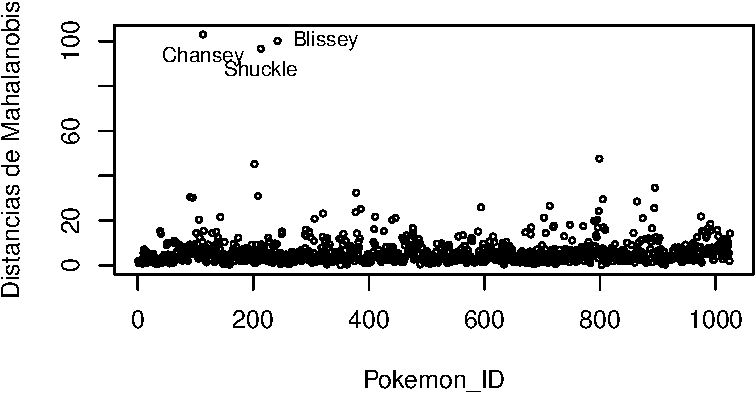
\includegraphics{trabajo_files/figure-pdf/unnamed-chunk-15-1.pdf}
\end{center}

Vemos además que la enorme mayoría de Pokémon pueden considerarse
``normales'', cercanos a la media según la distancia de Mahalanobis. Hay
algunas observaciones medianamente raras (con distancias entre 20 y 60);
y los tres Pokémon estudiados por separado son extremadamente raros.

\section{2.3. Estudio de los datos por
grupos}\label{estudio-de-los-datos-por-grupos}

Una vez hemos estudiado los datos sin agrupar, podemos agruparlos en
base a alguna de las variables categóricas antes mencionadas. Recordemos
que estas eran generación, tipo y categoría.

Quizás lo más interesante sea recurrir a los gráficos de correlaciones
del apartado anterior. Recordemos que gráficos como el de las variables
``total'' y ``attack'' parecían apuntar a la existencia de un grupo
reducido con características especialmente buenas.

\begin{quote}
Como curiosidad, recordemos que, en el análisis global, nos salía que
Chansey era el Pokémon más ``raro'' (lejano a la media), por su hp
extremadamente alto y un ataque y defensas extremadamente bajos. Podemos
etiquetarlo en este gráfico, para ver que sigue siendo un valor raro
dentro de los comunes (su ataque no es el que se esperaría de un Pokémon
con un ``total'' de 450).
\end{quote}

\begin{verbatim}
<environment: R_GlobalEnv>
\end{verbatim}

\begin{center}
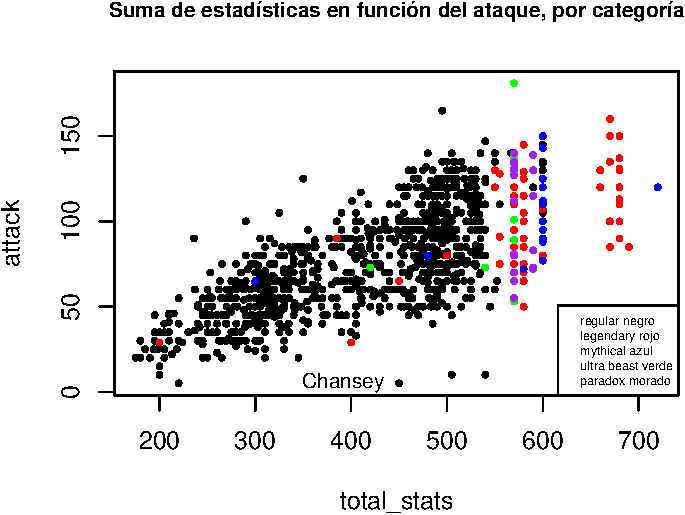
\includegraphics{trabajo_files/figure-pdf/unnamed-chunk-16-1.pdf}
\end{center}

Vemos que nuestra hipótesis parece correcta, y hemos elegido
aparentemente bien la variable categórica. El razonamiento ha sido que,
en el caso de existir algún grupo reducido de Pokémon poderosos,
deberían ser mucho más difíciles de conseguir. Aquí entran en juego las
categorías, ya que los Pokémon legendarios, singulares,
ultraentes\ldots{} son mucho más raros en general que los comunes.
Aunque la diferenciación entre Pokémon comunes y de otras categorías sí
es bastante clara (obviando unos pocos que se mezclan), vemos que los
legendarios, singulares, etc. se solapan en algunos puntos.

Con la información extraída del gráfico de correlación de ambas
variables, afirmamos:

\begin{itemize}
\item
  Hay muchos más Pokémon comunes que legendarios. Los más raros son los
  ultraentes, de los cuales solo hay unas pocas observaciones. Esta
  información es aplicable a la totalidad del dataset, para todas las
  variables.
\item
  Todos los singulares se concentran en valores de ``total'' alrededor
  de 600, y ataques bastante variados. No obstante, hay dos
  observaciones que se alejan mucho de esta cifra y quedan muy por
  debajo; y una que queda bastante por encima, coronándose como el
  Pokémon con mejores características globales. Veamos cuál es:

  \begin{table}[H]
  \centering\begingroup\fontsize{9.5}{11.5}\selectfont

  \begin{tabular}{llrrrrrrr}
  \toprule
    & name & total\_base\_stats & hp & attack & defense & special\_attack & special\_defense & speed\\
  \midrule
  493 & arceus & 720 & 120 & 120 & 120 & 120 & 120 & 120\\
  \bottomrule
  \end{tabular}
  \endgroup{}
  \end{table}
\item
  Vemos que el Pokémon singular que destaca es Arceus, el ``dios'' de
  los Pokémon en los juegos. Esto, junto con su categoría de Pokémon
  ``mítico'', explica por qué destaca como el mejor globalmente (todas
  sus estadísticas son bastante altas, pero no llegan tampoco a destacar
  individualmente, como vemos también en el valor de ``attack'' asociado
  a su valor en ``total'', que está alrededor del centro). El Pokémon
  con más ataque es un ultraente (coloreado en verde).

  \begin{figure}[H]

  {\centering 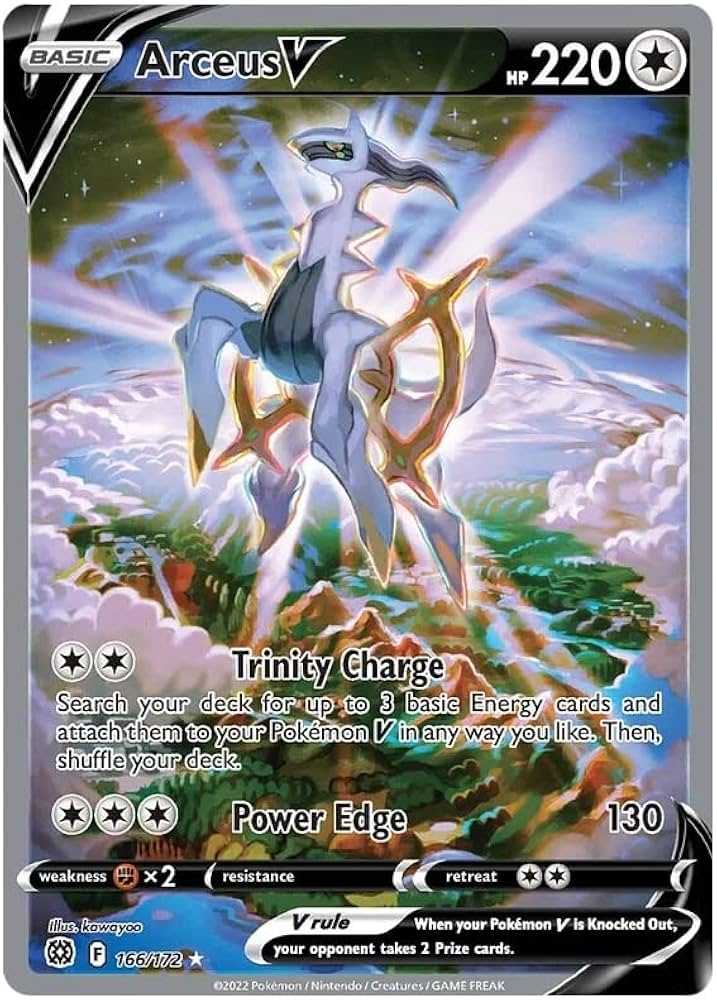
\includegraphics[width=2.23958in,height=\textheight]{trabajo_images/arceus_carta.jpg}

  }

  \caption{Carta especial de Arceus en el juego de cartas coleccionables
  de Pokémon (expansión Star Birth). Se representa como el concepto de
  deidad creadora en el que está basado. Se puede encontrar en Amazon
  por más de 180€ en castellano.}

  \end{figure}%
\item
  Los valores atípicos por abajo de estas categorías (Pokémon
  ``poderosos'') pueden deberse a que existen Pokémon que, a pesar de
  pertenecer a una categoría elevada, son ``formas base'' (que
  evolucionan a Pokémon con mejores características), por lo que sus
  estadísticas no son especialmente altas. Por ejemplo, veamos cuál es
  el ultraente que aparece entre los Pokémon comunes en el gráfico:

  \begin{table}[H]
  \centering\begingroup\fontsize{9.5}{11.5}\selectfont

  \begin{tabular}{llrrrrrrr}
  \toprule
    & name & total\_base\_stats & hp & attack & defense & special\_attack & special\_defense & speed\\
  \midrule
  803 & poipole & 420 & 67 & 73 & 67 & 73 & 67 & 73\\
  \bottomrule
  \end{tabular}
  \endgroup{}
  \end{table}

  Como decíamos, el Pokémon Poipole es un ultraente pero, a la vez, es
  una forma base. Evoluciona al Pokémon Naganadel, otro ultraente que ya
  sí pertenece al grupo de Pokémon poderosos (cerca de los 550 puntos en
  ``total'', y mejores estadísticas).

  \begin{table}[H]
  \centering\begingroup\fontsize{9.5}{11.5}\selectfont

  \begin{tabular}{llrrrrrrr}
  \toprule
    & name & total\_base\_stats & hp & attack & defense & special\_attack & special\_defense & speed\\
  \midrule
  804 & naganadel & 540 & 73 & 73 & 73 & 127 & 73 & 121\\
  \bottomrule
  \end{tabular}
  \endgroup{}
  \end{table}

  \begin{figure}[H]

  {\centering 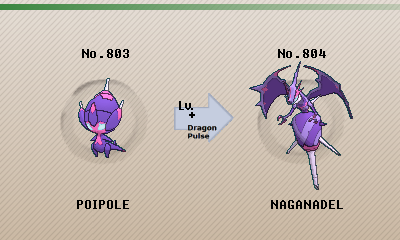
\includegraphics[width=3.125in,height=\textheight]{trabajo_images/Naganadel.png}

  }

  \caption{Línea evolutiva del ultraente Poipole, mostrando su evolución
  a Naganadel.}

  \end{figure}%
\end{itemize}

Este análisis lo hemos hecho con las variables ``total'' y ``attack'',
pero podríamos hacerlo con otras y obtendríamos resultados similares.
Observaremos esta diferencia sutil entre grupos en las correlaciones
donde interviene la variable ``total'', debido a que, a partir de los
550 puntos, casi todos los Pokémon son legendarios, míticos\ldots{} Para
mostrarlo, vamos a probar a hacer los diagramas de caja-bigotes para los
Pokémon separados por categoría para esta variable ``total'':

\begin{center}
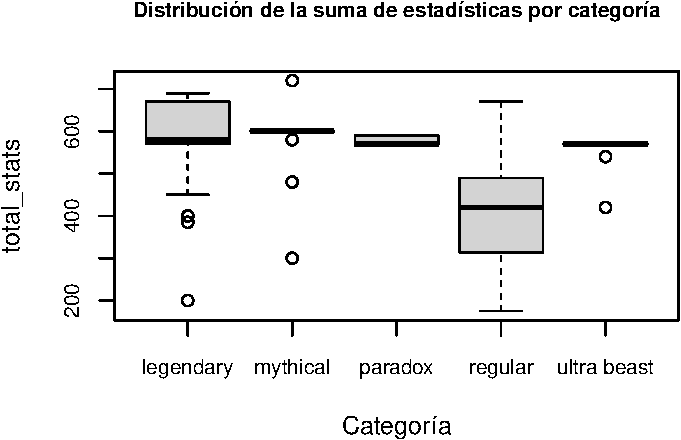
\includegraphics{trabajo_files/figure-pdf/unnamed-chunk-20-1.pdf}
\end{center}

\begin{quote}
Nota: Los atípicos observados en este estudio en la variable ``total''
lo son \textbf{para su grupo}, pero no para el dataset en general (ver
apartado 2.2).
\end{quote}

Vemos de nuevo que los Pokémon ``poderosos'' (legendarios, míticos,
paradox y ultraentes) tienden a quedar por encima de los comunes. Los
legendarios presentan una mayor variabilidad del valor global de las
estadísticas, pero los míticos, paradox y ultraentes apenas varían
(debido posiblemente a que son grupos muy reducidos). Los comunes, al
ser la amplia mayoría, presentan la mayor dispersión. Observamos lo
comentado ya con el análisis de ``total'' en función del ataque: hay
varios atípicos (respecto a la normal) en los grupos ``poderosos'' por
abajo, junto con el atípico identificado como Arceus por arriba en los
míticos.

El legendario más débil en cuanto a la variable ``total'' es el que
observamos en la esquina inferior izquierda de la nube de puntos:

\begin{table}[H]
\centering\begingroup\fontsize{9.5}{11.5}\selectfont

\begin{tabular}{llrrrrrrr}
\toprule
  & name & total\_base\_stats & hp & attack & defense & special\_attack & special\_defense & speed\\
\midrule
789 & cosmog & 200 & 43 & 29 & 31 & 29 & 31 & 37\\
\bottomrule
\end{tabular}
\endgroup{}
\end{table}

Se trata de Cosmog (de nuevo, legendario en forma base que puede
evolucionar a dos legendarios que sí siguen el comportamiento propio de
su grupo). Comprobamos si coincide con el legendario más raro según la
distancia de Mahalanobis:

\begin{table}[H]
\centering\begingroup\fontsize{9.5}{11.5}\selectfont

\begin{tabular}{lr}
\toprule
  & x\\
\midrule
895 & 27.10687\\
789 & 26.85396\\
377 & 22.30577\\
\bottomrule
\end{tabular}
\endgroup{}
\end{table}

Como podemos comprobar, si ordenamos el vector de distancias de
Mahalanobis tomando solo los Pokémon legendarios de la Pokédex, vemos
que Cosmog es la segunda observación más rara, con una distancia de
26.85396 a la media (su índice en la Pokédex es el 789, según la tabla
mostrada anteriormente). El más raro es el 895 (Regidraco).

\chapter{3. Análisis de Componentes
Principales}\label{anuxe1lisis-de-componentes-principales}

Continuaremos este estudio realizando un Análisis de Componentes
Principales (PCA) del vector aleatorio formado por las 7 variables
numéricas del dataset (desde ``total'' hasta ``speed''). Como hemos
mencionado en el análisis previo de los datos, podemos ver que, aunque
las variables hp, attack, defense, etc. toman valores en rangos
similares (escalas parecidas), la variable ``total'' rompe esta norma al
ser la suma de los valores de las demás. Por tanto, realizaremos el
análisis empleando la matriz de correlaciones en vez de la de
covarianzas, asignando a todas las variables la misma importancia.

Calcularemos por tanto las componentes principales como
\(Y_j = \hat{t}_j'X^*\), donde \(\hat{t}_j\) es el j-ésimo vector propio
de la matriz de correlaciones muestral \(P\) asociado a la j-ésima
componente principal; y \(X^*\) es el vector con las variables numéricas
estudiadas estandarizadas con la media y cuasivarianza muestrales. Así,
las medias de las variables serán 0 y las varianzas, 1. Llamaremos \(X\)
al vector aleatorio formado por las 7 variables numéricas del dataset.

\subsection{3.1. Cálculo de las componentes
principales}\label{cuxe1lculo-de-las-componentes-principales}

Comenzamos calculando las componentes principales de \(X^*\), y
mostrando un resumen sobre ellas. Al hacerlo, vemos que el valor propio
asociado a la última componente \(Y_7\) es nulo (varianza y desviación
típica nulas), por lo que podemos descartarla directamente y fijarnos en
las otras 6. Esta se anula ya que la variable ``total'' es suma de las
demaś (es una variable dependiente del resto).

\begin{verbatim}
[1] "Importance of components:"
\end{verbatim}

\begin{table}[H]
\centering
\caption{Resumen del PCA}
\centering
\fontsize{11}{13}\selectfont
\begin{tabular}[t]{lrrr}
\toprule
  & Desviación.Estándar & Proporción.de.Varianza & Proporción.Acumulada\\
\midrule
Comp.1 & 1.9085171 & 0.5203482 & 0.5203482\\
Comp.2 & 1.0514649 & 0.1579398 & 0.6782880\\
Comp.3 & 0.9392345 & 0.1260231 & 0.8043111\\
Comp.4 & 0.8198863 & 0.0960305 & 0.9003416\\
Comp.5 & 0.6514184 & 0.0606208 & 0.9609624\\
\addlinespace
Comp.6 & 0.5227457 & 0.0390376 & 1.0000000\\
Comp.7 & 0.0000000 & 0.0000000 & 1.0000000\\
\bottomrule
\end{tabular}
\end{table}

Lo primero que nos llama la atención es que la séptima componente no
contiene información sobre las variables de partida. Esto se debe a que
la variable ``total'' es la suma del resto de variables, con lo cual
depende de ellas (se puede obtener como combinación lineal). Por tanto,
la matriz de correlaciones muestral será semidefinida positiva, tendrá
un valor propio nulo, y es por ello que su componente principal asociada
no contiene información.

Con esta información, vamos a aplicar distintos criterios para ayudarnos
a decidir cuántas componentes principales vamos a estudiar en nuestro
análisis. Lo primero que podemos ver con el resumen ofrecido es la
proporción de información total mantenida por cada una (\emph{Proportion
of Variance}). Vemos que la primera contiene un 52.03\% de la
información de todas las variables iniciales en global. Si incluimos
también \(Y_2\), ya tendríamos un 67.83\%, y con \(Y_3\) la información
contenida ascendería a un 80.43\%. Estos dos últimos porcentajes podrían
parecernos suficiente de forma intuitiva. Calculamos las comunalidades
para cuantificar la información contenida por las 2 primeras componentes
sobre cada variable (suma de las saturaciones al cuadrado de \(Y_1\) e
\(Y_2\), para cada variable \(X_i\) estudiada):

\begin{table}[H]
\centering\begingroup\fontsize{11}{13}\selectfont

\begin{tabular}{lr}
\toprule
  & x\\
\midrule
total\_base\_stats & 0.9988654\\
hp & 0.4794716\\
attack & 0.5110709\\
defense & 0.7892175\\
special\_attack & 0.6278357\\
\addlinespace
special\_defense & 0.5428075\\
speed & 0.7987474\\
\bottomrule
\end{tabular}
\endgroup{}
\end{table}

Comprobamos que se mantiene casi el 100\% de información sobre
``total'', y más de un 75\% de defensa y velocidad. Tendríamos un
62.78\% de la información sobre el ataque especial, algo más de un 50\%
de defensa especial y ataque, y un 47.95\% de hp (la única que está por
debajo del 50\%, y aún así se acerca bastante). Parece ser que vamos a
tener suficiente información de todas las variables una a una, pero
aplicamos otros criterios para comprobarlo.

Podemos aplicar la regla del codo para estudiar el gráfico de
sedimentación que nos ayude a decidir cuántas componentes principales
puede ser interesante estudiar para que el análisis sea lo
suficientemente informativo y robusto:

\begin{center}
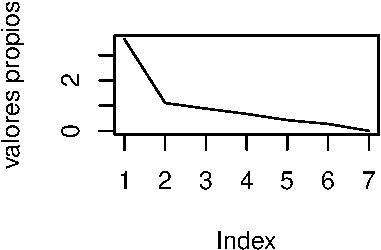
\includegraphics{trabajo_files/figure-pdf/unnamed-chunk-25-1.pdf}
\end{center}

Vemos claramente que el codo (los sedimentos) se encuentran en
\(j = 2\), lo que, según esta regla, nos llevaría a tomar únicamente la
primera componente. No obstante, dado que el estudio de las componentes
suele hacerse por parejas, para poder representar los gráficos
\texttt{biplot} y estudiar las características de los Pokémon en función
de la descripción que hagamos de cada componente (análisis), vamos a
trabajar con las dos primeras. Además, la segunda componente suele ser
más interesante y dar más juego, ya que suele dar unas características
más específicas aplicables a un grupo de Pokémon concreto.

Podemos mencionar que, si aplicamos la regla de Rao, obtenemos que las
componentes relevantes son las dos primeras. Esta regla establece que
las componentes relevantes para el análisis serán aquellas cuya
variabilidad (varianza, valor propio) sea superior al mínimo de las
cuasivarianzas muestrales de las variables originales con las que
calculamos las componentes. Dado que hemos usado las variables
estandarizadas \(X_i^*\), sus cuasivarianzas son 1. Si observamos el
resumen anterior de las componentes, vemos que las dos primeras son las
únicas que tienen desviaciones típicas (\(\sqrt{\lambda_j}\)) mayores
que 1 y, por tanto, varianzas mayores que 1.

Una vez decidido el número de componentes a considerar, pasamos a la
parte de análisis.

\subsection{3.2. Análisis de las componentes
principales}\label{anuxe1lisis-de-las-componentes-principales}

\subsubsection{\texorpdfstring{Primera componente
\(Y_1\)}{Primera componente Y\_1}}\label{primera-componente-y_1}

Hemos visto que esta componente contiene un 52.03\% de la información
inicial del vector de variables \(X\). Estudiamos los valores de las
cargas asociadas a \(Y_1\), es decir, el valor del vector propio de la
matriz de correlaciones muestrales, \(t_1\). Cada una de estas cargas
representa el peso o coeficiente que tiene la variable indicada en la
construcción de \(Y1\) como suma de las distintas \(X_i^*\). Tratamos de
asignar una interpretación a la variable \(Y_1\) en base al peso de cada
variable inicial:

\begin{table}[H]
\centering\begingroup\fontsize{10.5}{12.5}\selectfont

\begin{tabular}{lr}
\toprule
  & x\\
\midrule
total\_base\_stats & 0.5234776\\
hp & 0.3575828\\
attack & 0.3719660\\
defense & 0.3319564\\
special\_attack & 0.3672258\\
\addlinespace
special\_defense & 0.3739633\\
speed & 0.2735851\\
\bottomrule
\end{tabular}
\endgroup{}
\end{table}

Vemos que todas las variables (teniendo en cuenta que están
estandarizadas) tienen una influencia positiva en la construcción de la
componente. Así pues, un valor alto en \(Y_1\) implicará valores altos
en todas las variables iniciales estudiadas. La que más influye con
diferencia es la variable ``total'', por lo que un Pokémon para el cual
\(Y_1\) tome un valor alto será uno con alta suma de estadísticas (será
fuerte/poderoso en general). El resto de variables tienen influencias
(positivas) similares entre ellas, con pesos entre 0.33 y 0.38; excepto
speed, que influye algo menos. Por tanto, la primera componente puede
interpretarse como un indicador global de la fortaleza y competencia
general de un Pokémon, resumiendo sus capacidades y aptitudes en una
única medida.

Pasamos al análisis de las puntuaciones (\emph{scores}) de la
componente, es decir, los valores que toma \(Y_1\) para cada Pokémon.

\begin{verbatim}
   Min. 1st Qu.  Median    Mean 3rd Qu.    Max. 
-4.2786 -1.7600  0.3961  0.0000  1.3608  4.9173 
\end{verbatim}

Toma valores en la muestra (dataset) de entre -4.2786 y 4.9173, y tiene
media 0 al calcularse con las variables de partida estandarizadas. Puede
ser interesante también ver qué especies de Pokémon toman el máximo y
mínimo valor en \(Y_1\), es decir, según esta nueva medida general del
poder del Pokémon, cuál es el más y el menos poderoso.

El Pokémon donde \(Y_1\) alcanza el mayor valor es:

\begin{table}[H]
\centering\begingroup\fontsize{9.5}{11.5}\selectfont

\begin{tabular}{llrrrrrrr}
\toprule
  & name & total\_base\_stats & hp & attack & defense & special\_attack & special\_defense & speed\\
\midrule
493 & arceus & 720 & 120 & 120 & 120 & 120 & 120 & 120\\
\bottomrule
\end{tabular}
\endgroup{}
\end{table}

Nos encontramos de nuevo con el Pokémon deidad, Arceus. Es decir, el
Pokémon más poderoso globalmente coincide con el que hemos obtenido en
el análisis previo como el que mayor valor alcanza en su suma de
estadísticas (variable ``total'').

El Pokémon donde se alcanza el menor valor es:

\begin{table}[H]
\centering\begingroup\fontsize{9.5}{11.5}\selectfont

\begin{tabular}{llrrrrrrr}
\toprule
  & name & total\_base\_stats & hp & attack & defense & special\_attack & special\_defense & speed\\
\midrule
746 & wishiwashi & 175 & 45 & 20 & 20 & 25 & 25 & 40\\
\bottomrule
\end{tabular}
\endgroup{}
\end{table}

Se trata de Wishiwashi, un Pokémon de la séptima generación cuyas
estadísticas son bastante bajas en general, sin haber ningún desbalanceo
en especial. No obstante, Wishiwashi (cuya apariencia es la de un pez
pequeño, como un boquerón), tiene una ``forma banco'' en la que muchos
individuos de esta especie se unen para formar un Pokémon con apariencia
más temible y mejores estadísticas. Esta es una forma de compensar la
debilidad por la que destaca según esta componente \(Y_1\).

\begin{figure}[H]

{\centering 
\includegraphics[width=2.03125in,height=\textheight]{trabajo_images/wishiwashi.png}

}

\caption{Forma individual de Wishiwashi (derecha), el Pokémon
globalmente más débil según el análisis de la primera componentes
principal. A la izquierda, vemos su forma banco como algo más amenazador
y con mejores estadísticas.}

\end{figure}%

Si buscamos obtener el nombre del Pokémon que toma el menor valor en la
variable ``total'', nos sale también Wishiwashi. Por tanto, los
resultados obtenidos al estudiar los Pokémon en función de esta variable
parecen ser similares, si no iguales, a los obtenidos mediante el
estudio de \(Y_1\). Esto tiene sentido, ya que hemos visto que en la
construcción de \(Y_1\), es precisamente ``total'' la que más peso
tiene. Además, si \(Y_1\) es una medida de lo bueno que puede ser un
Pokémon según sus características, es de esperar que los resultados sean
similares a los que nos proporciona la variable ``total'' como suma del
resto de estadísticas. Podemos deducir que la componente \(Y_1\)
contendrá un gran porcentaje de la información de ``total'', cosa que
podemos ver calculando sus saturaciones al cuadrado:

\begin{table}[H]
\centering\begingroup\fontsize{10.5}{12.5}\selectfont

\begin{tabular}{lr}
\toprule
  & x\\
\midrule
total\_base\_stats & 0.9981327\\
hp & 0.4657419\\
attack & 0.5039628\\
defense & 0.4013785\\
special\_attack & 0.4912000\\
\addlinespace
special\_defense & 0.5093895\\
speed & 0.2726321\\
\bottomrule
\end{tabular}
\endgroup{}
\end{table}

Contiene un abrumador 99.81\% de la información de la variable
``total'', por lo que está casi totalmente representada.

\subsubsection{\texorpdfstring{Segunda componente
\(Y_2\)}{Segunda componente Y\_2}}\label{segunda-componente-y_2}

Repetimos el proceso para la segunda componente principal, comenzando
por el análisis y la asignación de significado a los pesos de cada
variable inicial en su construcción:

\begin{table}[H]
\centering\begingroup\fontsize{10.5}{12.5}\selectfont

\begin{tabular}{lr}
\toprule
  & x\\
\midrule
total\_base\_stats & 0.0257434\\
hp & -0.1114387\\
attack & -0.0801824\\
defense & -0.5922853\\
special\_attack & 0.3515502\\
\addlinespace
special\_defense & -0.1738582\\
speed & 0.6898358\\
\bottomrule
\end{tabular}
\endgroup{}
\end{table}

En el caso de \(Y_2\), parece que las influencias son un poco más
variadas y pueden ser más interesantes en su análisis. Destacan como
variables con alta influencia la velocidad (positiva), y la defensa
(negativa). En menor medida, el ataque especial influye positivamente, y
la defensa especial lo hace de manera negativa. Podríamos decir que el
ataque y la variable ``total'' no influyen, y hp parece tener poca
importancia también.

Así pues, \(Y_2\) tomará valores grandes en Pokémon veloces y con poca
defensa (e incluso quizás con ataques especiales que causen bastante
daño). Únicamente con la interpretación de estos pesos, podemos imaginar
algunos prototipos de Pokémon cuya forma de combatir se ajuste a estas
características: aquellos de complexión o construcción ligera, facilidad
de movimiento, precisión para atacar de forma rápida y potente\ldots{} A
cambio de ser más difíciles de alcanzar, recibir un ataque podrá ser
fatal para ellos debido, precisamente, a la baja defensa.

Si tenemos un conocimiento algo más profundo sobre el tema, podemos
incluso darnos cuenta de que estas características suelen corresponderse
con Pokémon de tipo eléctrico o psíquico, dado que sus ``elementos'' se
caracterizan por su velocidad de transmisión. Podemos verlo
intuitivamente en el caso de Pokémon eléctricos: dado que la
electricidad se propaga de forma muy rápida, tiene sentido físico que
sus rasgos les permitan moverse y atacar con agilidad. En el otro
extremo, tendrá sentido que los Pokémon de tipo roca se muevan de forma
mucho más lenta, pero que tengan mucha más defensa. Podemos pensar que
estos tomarán valores más pequeños en \(Y_2\).

Analizamos las puntuaciones (\emph{scores}) de \(Y_2\):

\begin{verbatim}
    Min.  1st Qu.   Median     Mean  3rd Qu.     Max. 
-6.02742 -0.59034  0.05033  0.00000  0.66635  4.06726 
\end{verbatim}

Toman valores entre -6.03 y 4.07, de nuevo con media 0 como la primera.
Esto nos da una medida numérica en este rango que describe cómo se
ajustan las características de un Pokémon al perfil descrito. Estudiamos
cuáles son los que más y menos encajan en este prototipo, que
resumiremos como ``golpeadores ágiles''.

El nombre y tipo del Pokémon más ágil es:

\begin{table}[H]
\centering\begingroup\fontsize{10.5}{12.5}\selectfont

\begin{tabular}{lll}
\toprule
  & name & primary\_type\\
\midrule
894 & regieleki & electric\\
\bottomrule
\end{tabular}
\endgroup{}
\end{table}

Ponemos sus características numéricas para que todas sean visibles:

\begin{table}[H]
\centering\begingroup\fontsize{9.5}{11.5}\selectfont

\begin{tabular}{lrrrrrrr}
\toprule
  & total\_base\_stats & hp & attack & defense & special\_attack & special\_defense & speed\\
\midrule
894 & 580 & 80 & 100 & 50 & 100 & 50 & 200\\
\bottomrule
\end{tabular}
\endgroup{}
\end{table}

Vemos que, en efecto, toma el máximo valor para la velocidad, la defensa
destaca por ser especialmente baja, y el valor de ataque especial es
relativamente alto. Además, es de tipo eléctrico, lo cual coincide con
nuestro razonamiento previo, extrapolando las características a los
elementos del ``mundo real''.

Los 3 Pokémon donde \(Y_2\) toma menor valor son:

\begin{table}[H]
\centering\begingroup\fontsize{10.5}{12.5}\selectfont

\begin{tabular}{lll}
\toprule
  & name & primary\_type\\
\midrule
213 & shuckle & bug\\
805 & stakataka & rock\\
208 & steelix & steel\\
\bottomrule
\end{tabular}
\endgroup{}
\end{table}

Recordemos que Shuckle había aparecido antes como un Pokémon raro (junto
a Chansey y Blissey), debido a su altísima defensa. Vamos a ver el resto
de características de estos Pokémon, encontrando velocidades bajas y
defensas muy altas, junto con un ataque especial también relativamente
bajo:

\begin{table}[H]
\centering\begingroup\fontsize{9.5}{11.5}\selectfont

\begin{tabular}{lrrrrrrr}
\toprule
  & total\_base\_stats & hp & attack & defense & special\_attack & special\_defense & speed\\
\midrule
213 & 505 & 20 & 10 & 230 & 10 & 230 & 5\\
805 & 570 & 61 & 131 & 211 & 53 & 101 & 13\\
208 & 510 & 75 & 85 & 200 & 55 & 65 & 30\\
\bottomrule
\end{tabular}
\endgroup{}
\end{table}

Es curioso ver que, respecto a nuestras suposiciones iniciales sobre los
tipos, Stakataka es de tipo roca, pero Shuckle y Steelix tiene el tipo
roca como tipo secundario (aunque se ha prescindido de él en el
estudio).

\begin{figure}[H]

{\centering 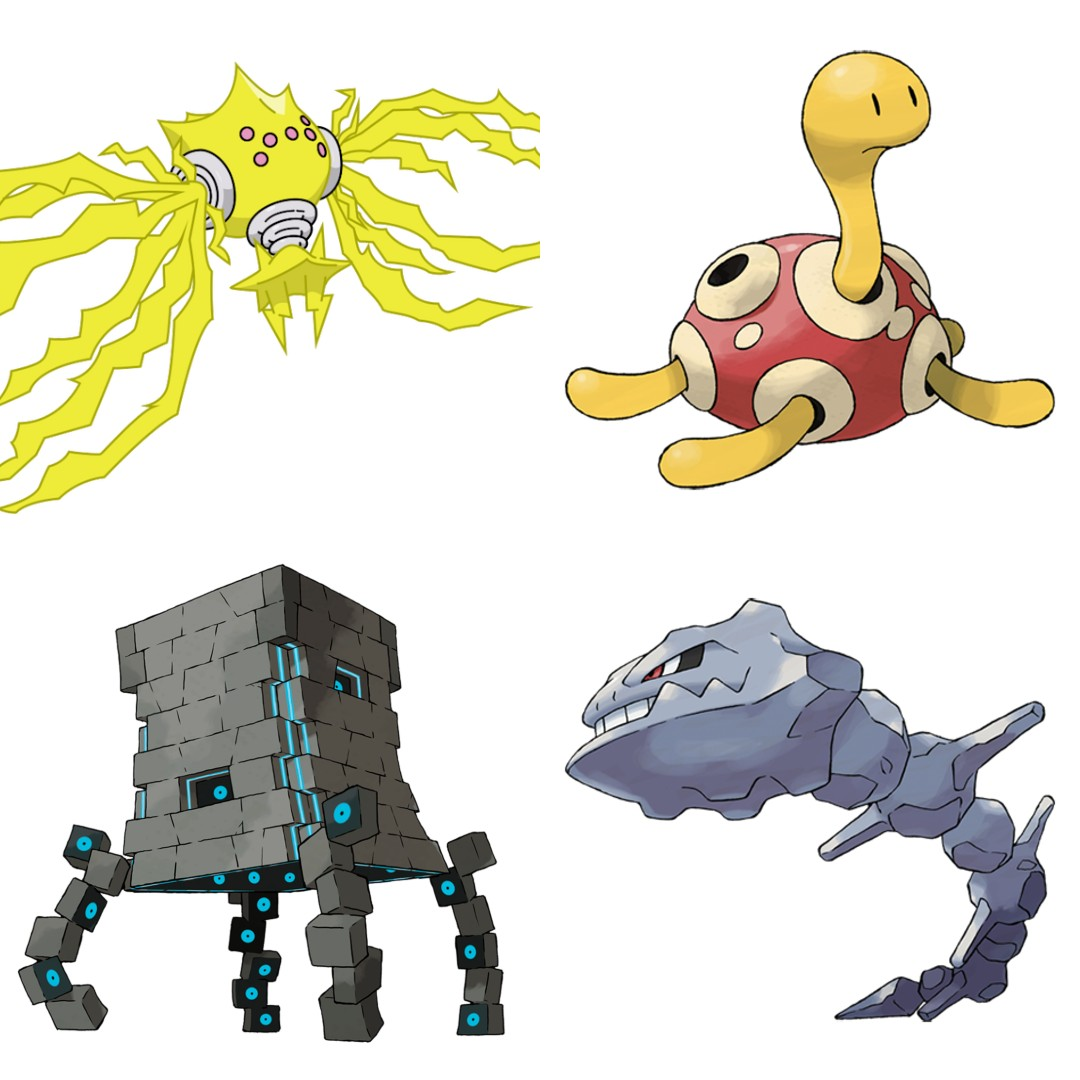
\includegraphics[width=2.86458in,height=\textheight]{trabajo_images/pokemons.jpg}

}

\caption{De izquierda a derecha y de arriba a abajo: Regieleki, cuyo
diseño está basado en una bobilla y representa al tipo eléctrico;
Shuckle, de tipo bicho y roca, similar a un caracol; Stakataka, de tipo
roca, similar a un monolito con patas; y Steelix, de tipo acero y roca.
La apariencia de todos va de la mano de las características que podemos
extraer según la construcción de \(Y_2\) y el valor que toma para cada
uno.}

\end{figure}%

Esto pone de manifiesto la influencia que tienen las características
numéricas de un Pokémon en otros aspectos que, a priori, no deberían
tener relación directa, como pueden ser su tipo o su diseño artístico.
Es increíble cómo, a través del análisis de las componentes principales
(sobre todo de \(Y_2\)), hemos podido extraer grupos de Pokémon con unos
rasgos muy marcados que nos han permitido deducir a qué tipo tendría
sentido que pertenecieran, antes incluso de estudiarlos uno a uno.

Además, la figura 5 muestra claramente cómo estos rasgos hacen que el
Pokémon tenga un diseño u otro, para transmitir visualmente lo que se
puede estudiar de manera numérica. Ejemplo de ello es Shuckle, que, por
ser el de menor valor de \(Y_2\), según nuestro análisis será un Pokémon
con muy buena defensa, movimientos lentos, resistente, poco ágil\ldots{}
Al ver su diseño, este adquiere un sentido más allá de la simple
estética: el hecho de estar basado en un caracol (que es algo cotidiano
a lo que inconscientemente asignamos los rasgos de lentitud y caparazón
resistente) está perfectamente pensado para representar visualmente las
características descritas a través del bajo valor de \(Y_2\).

\subsubsection{Análisis conjunto en
gráfica}\label{anuxe1lisis-conjunto-en-gruxe1fica}

Una vez tratadas \(Y_1\) e \(Y_2\) por separado, y habiéndoles asignado
un significado a sus valores, podemos representar gráficamente ambas
para ver lo que hemos descrito y analizar sus interacciones. Dado que el
\texttt{biplot} implementado por R etiquetará a todos los Pokémon por su
índice o nombre, y hay 1025, no se verán bien. Lo mostramos aun así para
poder observar gráficamente al menos los vectores que representan la
influencia de cada variable en cada componente. Comprobaremos así lo
descrito con más detalle en sus correspondientes apartados.

\begin{center}
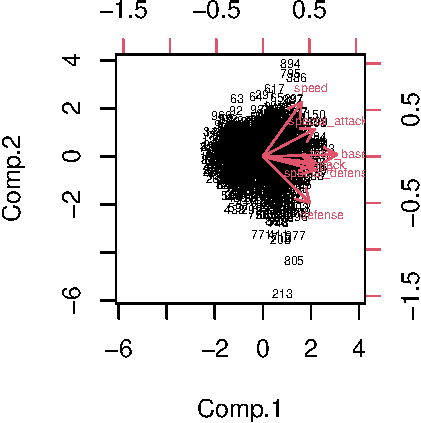
\includegraphics{trabajo_files/figure-pdf/unnamed-chunk-37-1.pdf}
\end{center}

Como decíamos, solo podemos distinguir correctamente a los que toman
valores más entremos de las componentes. No obstante, si nos fijamos en
los vectores que representen la influencia de cada variable en \(Y_1\) e
\(Y_2\), podemos observar las características ya comentadas. Primero,
todas las variables están bien representadas en estas dos componentes
dado que los vectores son largos (cosa que veíamos con la información
que contienen tanto en general como con las comunalidades). Vemos la
influencia positiva de todas las variables en \(Y_1\) (valores altos en
estas implicarán un valor alto en la componentes), siendo ``speed'' la
que menos influye. Por su parte, podemos comprobar que las únicas que
parecen tener una influencia digna de mención en \(Y_2\) son la
velocidad (positiva), la defensa (negativa) y, en menor medida, el
ataque especial (positiva). Esto nos conduce a la interpretación dada en
su correspondiente apartado.

Para analizar los datos en sí (a los Pokémon en general), optamos por
hacer un gráfico sólo de las puntuaciones sin estandarizar de las dos
primeras componentes, y localizar en él los Pokémon que hemos mencionado
a lo largo del análisis.

\begin{quote}
Nota: Habría sido interesante representar en este gráfico los tipos con
distintos colores, pero, al hacerlo, se ha visto que el elevado número
de tipos entorpece la interpretación del gráfico. Además, la influencia
del tipo secundario en la relación comentada entre \(Y_2\) y el tipo del
Pokémon hace que perdamos información y no percibamos ningún patrón
destacable.
\end{quote}

\begin{center}
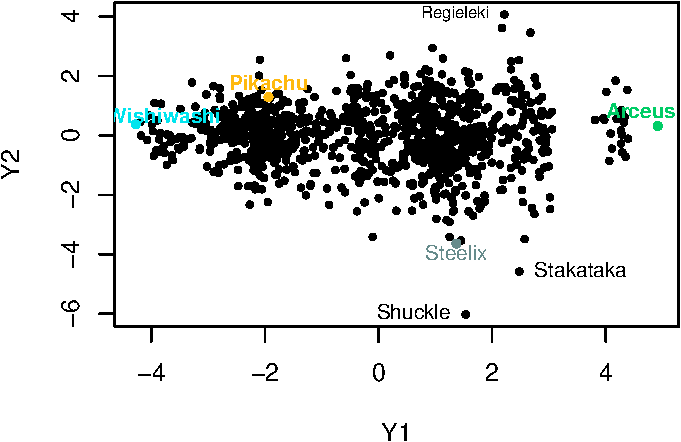
\includegraphics{trabajo_files/figure-pdf/unnamed-chunk-38-1.pdf}
\end{center}

Como la componente \(Y_1\) está en el eje horizontal, cuanto más a la
derecha esté un Pokémon, significará que sus características en general
son mejores, sobre todo en cuanto a la variable ``total''. De hecho, si
solo prestamos atención a la distribución ``en horizontal'', es muy
similar a la observada en otras gráficas anteriores donde hemos
estudiado la variable ``total''. Por su parte, \(Y_2\) está en el eje
vertical, por lo que cuanto más arriba esté un Pokémon, significará que
es más ágil moviéndose y atacando, y tendrá menos defensa (y al revés:
cuanto más abajo, más estático o lento será y más defensa tendrá).

Podemos decir que el poder o fortaleza general de los Pokémon (valor de
\(Y_1\)) está bastante equilibrado, ya que las observaciones se reparten
a lo largo de todo el eje horizontal. En \(Y_2\), los Pokémon se
concentran más en torno al 0 (media), y conforme nos alejamos de ese
valor, las observaciones son más escasas. Esto nos indica que no son
muchos los Pokémon que destaquen por ser muy ágiles o muy resistentes:
la mayoría son un término medio entre ambos perfiles. Los que destacan
por un extremo u otro tienden a tomar valores centrales (quizás por
arriba) en \(Y_1\).

En cuanto a los Pokémon marcados, Arceus vuelve a estar algo aislado a
la cabeza (punto más a la derecha de la gráfica), pero toma un valor muy
cercano a la media en \(Y_2\), por lo que no destaca ni por su agilidad
ni por su defensa (está equilibrado en ese sentido, ninguna de las
características que influyen en \(Y_2\) destaca). Lo mismo ocurre con
Wishiwashi, sólo que este está completamente a la izquierda como Pokémon
de peores estadísticas en general (menor \(Y_1\) y menor valor de
``total'').

También hemos marcado a los Pokémon comentados en el análisis de \(Y_2\)
como más ágiles (Regieleki) y los menos ágiles y más resistentes
(Shuckle, Stakataka\ldots). Vemos que, en cuanto a \(Y_1\), los 4 toman
valores algo por encima de la media, por lo que, en términos generales,
pueden considerarse poderosos. No obstante, estos ``términos generales''
pueden ser peligrosos, ya que hemos visto por la construcción de \(Y_2\)
que valores extremos en estas componentes indican un desbalanceo en las
estadísticas velocidad-defensa (principalmente). Que tomen valores
medianamente altos en \(Y_1\) y, por tanto, en ``total'', puede ser
resultado de una velocidad o defensa anormalmente altas. Esto nos indica
que no podemos guiarnos únicamente por lo bueno que sea un Pokémon ``en
general'' a la hora de evaluarlo.

Por último, como curiosidad y aplicación práctica de esta sección, hemos
marcado al conocido Pokémon de tipo eléctrico Pikachu (punto amarillo),
que se ha convertido en el representante de la franquicia y en un
símbolo a nivel cultural. Sólo observando su posición, podemos
imaginarnos cómo va a ser sin necesidad de ver sus estadísticas
específicas. Por un lado, toma un valor bastante por debajo de la media
en \(Y_1\), lo que indica que, en general, no destaca por tener unas
estadísticas altas. En \(Y_2\), se encuentra por encima de la media, lo
que lo hace un Pokémon más rápido que resistente. Esto cuadra con el
perfil de Pikachu como Pokémon roedor que, además, vuelve a ser de tipo
eléctrico (habíamos dicho que, normalmente, este tipo es el que más se
ajusta al perfil de Pokémon ágil con poca defensa).

Esto demuestra que podríamos identificar en la gráfica cualquier Pokémon
que se nos ocurra, y con un simple vistazo, hacernos una idea bastante
precisa acerca de sus características y comportamiento sin necesidad de
estudiarlas detenidamente. Aquí reside la potencia y utilidad de este
análisis, que termina simplificando el estudio de un conjunto de datos
denso asignando un significado a la interacción de las variables.

\chapter{4. Análisis Cluster}\label{anuxe1lisis-cluster}

\section{4.1. Introducción y consideraciones
previas}\label{introducciuxf3n-y-consideraciones-previas}

Aunque ya hemos estudiado en secciones anteriores pequeñas
diferenciaciones de Pokémon por grupos, quizá puede ser interesante
analizar toda la Pokédex para tratar de encontrar similitudes ocultas o
no observables tan intuitivamente. De esta forma, podemos preguntarnos
si hay algún criterio no considerado en el dataset que nos permita
distinguir Pokémon por clases (más allá de criterios del dataset como
tipo, categoría\ldots).

Para desarrollar esto, lo primero que tenemos que preguntarnos es, en
caso de buscar una separación de Pokémon por nuevos grupos, ¿cuántos
deberíamos distinguir? Dependiendo de esto, la interpretación de cada
uno (es decir, las características de los Pokémon incluidos en un grupo
u otro) podrá cambiar drásticamente. Antes de hacer nada, se nos pueden
ocurrir algunas separaciones intuitivas. De más trivial a más compleja:

\begin{itemize}
\item
  Pokémon ``poderosos'' en general frente a Pokémon más débiles (algo
  similar a lo visto en el apartado 2, o mediante la primera componente
  principal).
\item
  Separación más profunda de estadísticas: dividir los Pokémon por los
  que destaquen en ataque (y ataque especial), en defensa (y defensa
  especial), en salud (``hp'') o en velocidad.
\item
  Separación por tantos grupos como tipos haya (18), para ver si podemos
  percibir diferencias entre tipos a nivel de características.
\end{itemize}

Como podemos ver, hay muchas opciones para enfocar este apartado. Antes
de nada, recordemos que la variable ``total'' es calculada a partir de
la suma de los valores de las otras 6 variables numéricas en cada
Pokémon. Para formar los grupos, es altamente conveniente quitarla, dado
que podría acaparar la variabilidad y hacer que la creación de grupos
dependa demasiado de ella. Por tanto, en este apartado trabajaremos con
un dataset en el que obviamos esta variable.

Además, hemos visto en el apartado de análisis previo que el resto de
variables tienen escalas muy similares. No obstante, trabajaremos con
los datos estandarizados para mayor claridad, dado también que hay
muchos atípicos en todas estas variables y queremos asegurarnos de que
todas tienen el mismo peso para obtener una división por grupos
satisfactoria. Para estandarizar los datos, ejecutamos este comando en
R, trabajando ahora con el dataset \texttt{ds}:

\begin{Shaded}
\begin{Highlighting}[]
\NormalTok{ds }\OtherTok{\textless{}{-}} \FunctionTok{data.frame}\NormalTok{(}\FunctionTok{scale}\NormalTok{(d[}\DecValTok{6}\SpecialCharTok{:}\DecValTok{11}\NormalTok{]))}
\end{Highlighting}
\end{Shaded}

Dado que el análisis de componentes principales anterior lo hemos hecho
incluyendo la variable ``total'', no está claro si sería aplicable para
interpretar los grupos que hagamos en este apartado (si bien nos ha
ayudado a detectar relaciones importantes entre los datos, a modo de
exploración). Vamos a realizar un pequeño PCA adicional quitando la
variable ``total'', para estudiar qué cambia respecto del anterior.
Realizaremos únicamente el \texttt{biplot}, ofreciendo una
interpretación rápida de las nuevas dos primeras componentes, \(Y_1'\) e
\(Y_2'\), y de lo más destacable que observemos:

\begin{center}
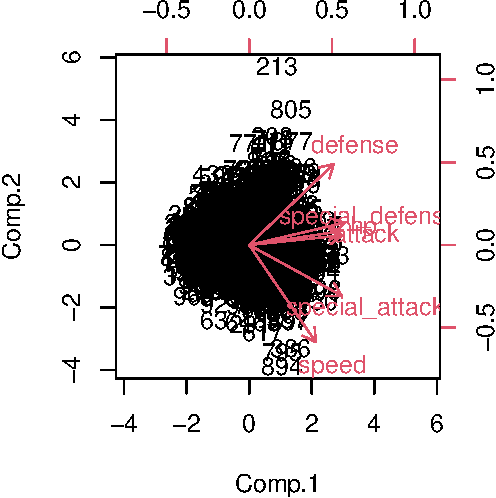
\includegraphics{trabajo_files/figure-pdf/unnamed-chunk-40-1.pdf}
\end{center}

Podemos observar claramente que la nueva primera componente tendría una
interpretación muy similar a la \(Y_1\) del apartado anterior, aun
prescindiendo de ``total\_base\_stats''. Todas las variables influyen
positivamente en ella, siendo ``speed'' la que menos lo hace, tal y como
ocurría en el apartado anterior. Es, de nuevo, una medida de cuán
``poderoso'' en general es un Pokémon.

Por otro lado, si nos fijamos en \(Y_2'\), vemos que su interpretación
es idéntica a la de \(Y_2\) sólo que al revés (los ``loadings'' en este
PCA saldrán cambiados de signo con respecto a los del anterior). Ahora,
la defensa tiene una influencia positiva en la componente, y la
velocidad (y el ataque especial en menor medida) influyen negativamente.
Esto se ve también en los Pokémon que toman valores extremos en
\(Y_2'\), que son los mismos que mencionábamos en \(Y_2\) pero cambiando
el signo de sus puntuaciones. Así, el Pokémon 213 (Shuckle), que
aparecía en la parte inferior de la gráfica del anterior PCA como un
Pokémon más resistente, figura ahora en la parte superior, teniendo la
misma interpretación. Lo mismo ocurre con el resto de Pokémon
mencionados anteriormente.

Vemos, por tanto, que el cálculo e interpretación de las componentes
principales no cambian drásticamente y podemos recurrir al análisis del
punto anterior para enriquecer el proceso de \emph{clustering} en caso
de verlo necesario.

\section{4.2. Caso práctico}\label{caso-pruxe1ctico}

Para darle una nueva dimensión a esta técnica, vamos a realizar el
análisis cluster enfocándonos en un problema concreto. Imaginemos que un
jugador dispone de todos los Pokémon en la Pokédex para construir un
equipo, pero sólo tiene claro que quiere incluir ciertas especies en
concreto. Sería interesante implementar un sistema de recomendación
automática de Pokémon para autocompletar un equipo, que típicamente
viene formado por 6 criaturas.

El objetivo de este apartado será, a partir de un ejemplo concreto,
detallar el proceso que se seguiría para conseguir una lista de
recomendaciones de Pokémon que se complementen o funcionen bien con unos
pocos Pokémon dados. Conseguiremos esto valiéndonos del análisis cluster
del dataset con todas las especies. A pesar de que se irá siguiendo el
ejemplo, la idea es que exactamente el mismo procedimiento sea aplicable
para cualquier caso, obteniendo finalmente un método relativamente
fiable para aconsejar a un jugador cualquiera que no sepa cómo completar
su equipo. Partiremos del equipo incompleto de 5 Pokémon formado por:

\begin{itemize}
\item
  Lucario, Pokémon número 448 en la Pokédex, de tipo Lucha y Acero, que
  destaca en ataque físico y especial, además de tener una velocidad
  decente.
\item
  Mewtwo, número 150 en la Pokédex, legendario de tipo Psíquico, con
  altísimas estadísticas de ataque especial y velocidad.
\item
  Greninja, número 658, de tipo Agua y Siniestro, con una velocidad
  excepcional y buenos valores de ataque especial.
\item
  Excadrill, número 530, de tipo Tierra y Acero, que destaca como
  atacante físico.
\item
  Haxorus, número 612, de tipo Dragón, que destaca por tener uno de los
  mejores valores para ataque físico.
\end{itemize}

Observamos sus características más en detalle:

\begin{table}[H]
\centering\begingroup\fontsize{10.5}{12.5}\selectfont

\begin{tabular}{llrrrrrr}
\toprule
  & name & hp & attack & defense & special\_attack & special\_defense & speed\\
\midrule
448 & lucario & 70 & 110 & 70 & 115 & 70 & 90\\
150 & mewtwo & 106 & 110 & 90 & 154 & 90 & 130\\
658 & greninja & 72 & 95 & 67 & 103 & 71 & 122\\
530 & excadrill & 110 & 135 & 60 & 50 & 65 & 88\\
612 & haxorus & 76 & 147 & 90 & 60 & 70 & 97\\
\bottomrule
\end{tabular}
\endgroup{}
\end{table}

Vemos que, dada la distribución de estadísticas que hemos observado en
el análisis inicial, estos Pokémon toman valores alrededor de la media
en puntos de salud (``hp''), defensa, y defensa especial, y destacan
sobre todo por sus altos valores en ataque y ataque especial, yendo esto
acompañado de velocidades realmente altas. Parece que el equipo que
pretende formar el entrenador está orientado sobre todo a la velocidad y
el ataque. Los Pokémon que lo componen de momento tomarían el rol, en
general, de ``atacantes rápidos''.

\begin{figure}[H]

{\centering 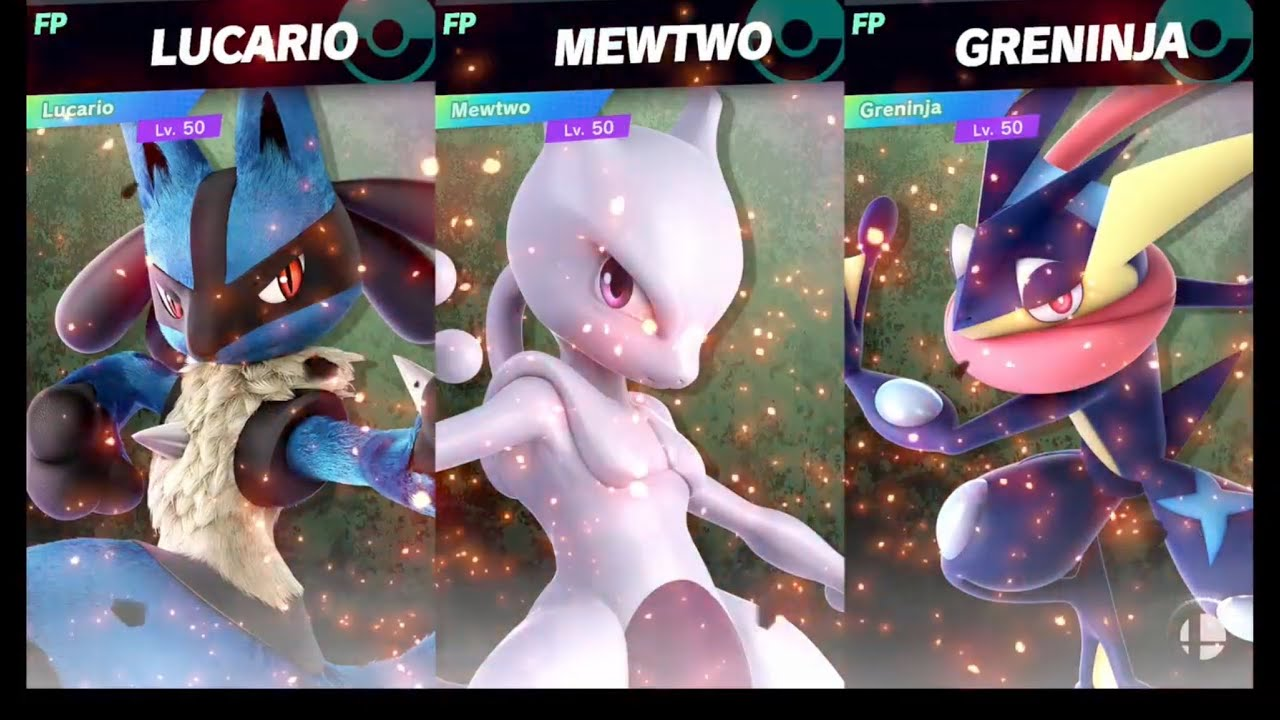
\includegraphics[width=3.90625in,height=\textheight]{trabajo_images/lucario_gren_mewtwo.jpg}

}

\caption{Lucario, Greninja y Mewtwo, tres de los Pokémon que se incluyen
en este equipo hipotético que debemos completar. La imagen viene del
videojuego de lucha \emph{Super Smash Bros Ultimate}, de Nintendo, donde
se introducen estos Pokémon como personajes jugables.}

\end{figure}%

Lo primero que deberíamos preguntarnos es cómo autocompletar el equipo,
es decir, en base a qué criterio podemos decir que un Pokémon es
``mejor'' que otro para formar parte de este. Dado que queremos hacer
del estudio algo simple dentro de lo que cabe, vamos a centrarnos en
tomar la decisión en base a las 6 variables numéricas que estamos
manejando. Así, podemos definir dos criterios:

\begin{enumerate}
\def\labelenumi{\arabic{enumi}.}
\item
  Recomendar Pokémon \textbf{similares} a los que ya hay en el equipo.
  Esta opción sería buena si buscamos homogeneizarlo, de forma que se
  especialice en un estilo de combate concreto. En este caso, este
  criterio implicaría buscar otros Pokémon con características similares
  a los dados, ya que funcionarían bien en la estrategia de combate más
  ofensiva que el jugador podría estar buscando.
\item
  Recomendar Pokémon \textbf{distintos} a los que se nos dan, buscando
  un enfoque de complementariedad. Es decir, si observamos que un equipo
  tiende a incluir Pokémon de unas características determinadas, dejando
  otras de lado, podríamos ofrecer como opción un Pokémon que equilibre
  el equipo. En este caso, eso implicaría considerar la opción de
  incluir algún Pokémon más robusto, que quizás destaque en defensa y
  puntos de salud.
\end{enumerate}

Ambas opciones tienen sentido y pueden ser de utilidad dependiendo de lo
que el cliente (el jugador, en este caso) busque, por lo que vamos a
tratar de implementar las dos. Tenemos por tanto como objetivo final
devolver dos listas de Pokémon, cada una ofreciendo recomendaciones para
rellenar el hueco en base a cada uno de los criterios. En un análisis
real, habría que tener en cuenta compatibilidades en cuanto a tipos,
rareza, debilidades o habilidades específicas\ldots{} Podemos tomar lo
que se va a hacer a continuación como un punto de partida rudimentario.

El primer paso sería realizar un \emph{clustering} general,
distinguiendo una serie de grupos para definir los criterios de
similitud entre Pokémon. Vamos a basarlo en el método de K-means, debido
a que en futuros pasos, trataremos el equipo como un pseudo-individuo
(es decir, como si fuera un nuevo Pokémon que representara los cinco que
tenemos), y querremos ver en qué grupo estaría. No obstante, para la
asignación de Pokémon similares, es posible que apoyarnos del
\emph{clustering jerarquizado} pueda sernos útil también.

\subsection{Agrupación inicial con
K-means}\label{agrupaciuxf3n-inicial-con-k-means}

Después de algunas pruebas, se ha optado finalmente por distinguir
\(K = 4\) grupos, dado que una clasificación en 2 grupos da lugar a
criterios como el primero que hemos mencionado, y sería demasiado
general. No obstante, aumentar demasiado \(K\) termina atomizando
demasiado los grupos y haciendo que las diferencias entre ellos sean
demasiado sutiles.

Mostramos a continuación la información de los centroides obtenidos, y
la distinción de los grupos en el gráfico de puntuaciones de las dos
primeras componentes principales (nota: tras algunas pruebas, en las que
se ha considerado también trabajar con la tercera o la cuarta componente
principal, se ha detectado que este gráfico es en el que mejor se
distinguen los grupos, aunque hay cierto solapamiento debido a la
pérdida de información al proyectar las variables en dos dimensiones).

\begin{table}[H]
\centering\begingroup\fontsize{11.5}{13.5}\selectfont

\begin{tabular}{lrrrr}
\toprule
  & C1 & C2 & C3 & C4\\
\midrule
hp & 0.4403366 & -0.7741951 & -0.0144998 & 0.9459595\\
attack & 0.6983985 & -0.8195241 & 0.3201562 & 0.3244725\\
defense & 1.0731435 & -0.7453431 & -0.2425586 & 0.3896001\\
special\_attack & -0.2444661 & -0.7451537 & 0.3696387 & 1.2726173\\
special\_defense & 0.3821320 & -0.8026841 & -0.0286370 & 1.0872740\\
\addlinespace
speed & -0.4162411 & -0.6208606 & 1.0407767 & 0.4576889\\
\bottomrule
\end{tabular}
\endgroup{}
\end{table}

\begin{center}
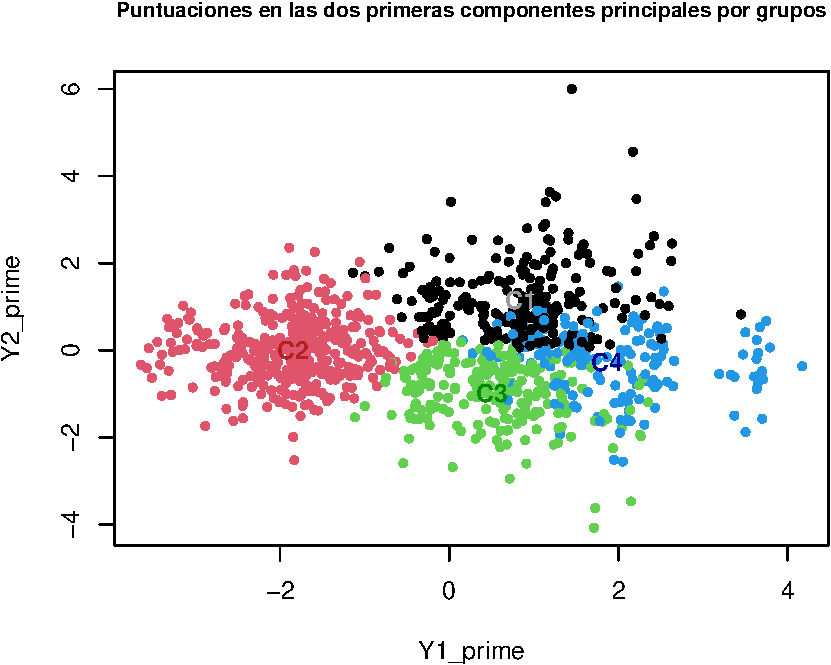
\includegraphics{trabajo_files/figure-pdf/unnamed-chunk-43-1.pdf}
\end{center}

Gracias a los representantes de cada grupo y al análisis de la gráfica,
donde también hemos incluido las proyecciones de los centroides según
las dos primeras componentes, podemos detallar las características de
cada grupos:

\begin{itemize}
\item
  \textbf{Grupo 1 (negro)}: Destaca por una defensa muy por encima de la
  media, junto con una defensa especial, ataque y puntos de salud
  medios/altos. Esto explica que los individuos de este grupo sean los
  que toman valores altos y alrededor de la media por arriba en
  \(Y_2'\). Serán \textbf{Pokémon más robustos y resistentes (tanques)}
  en general (en el apartado anterior, hemos visto que son algunos de
  tipo Roca como Shuckle). Toma valores medios/altos en \(Y_1'\), por lo
  que podremos decir que los Pokémon del grupo tendrán una tendencia al
  equilibrio en términos de poder general.
\item
  \textbf{Grupo 2 (rojo)}: Observamos que incluye Pokémon con valores
  bajos de \(Y_1'\), y su centroide tiene valores bastante por debajo de
  la media en todas las estadísticas. Podemos resumir los Pokémon en
  este cluster como \textbf{Pokémon débiles}. En el gráfico con las
  componentes principales, es el grupo que más claramente se separa de
  los demás.
\item
  \textbf{Grupo 3 (verde)}: Parece el opuesto del primero, creado en
  base a la separación de Pokémon por los valores en \(Y_2'\). Tanto por
  el significado de esta componente como por los valores observados en
  el centroide, podemos definir el grupo como el de \textbf{Pokémon muy
  veloces y ofensivos}, dado que vemos que están muy por encima de la
  media en cuanto a velocidad y muy por debajo en cuanto a defensa. Es
  por esto que son los que toman valores bajos en \(Y_2'\) (según el
  apartado anterior, eran algunos de tipo eléctrico como Regieleki), y
  el ataque y ataque especial están algo por encima de la media,
  quedando los puntos de salud y la defensa especial alrededor de la
  media. Por los valores medios/altos en \(Y_1'\), también podemos decir
  que no destacarán por ser muy poderosos en general (ni por quedar muy
  por debajo).
\item
  \textbf{Grupo 4 (azul)}: Son Pokémon que se caracterizan por tomar un
  valor alto en \(Y_1'\), estando por encima de la media en todas las
  características, destacando ``hp'', ataque especial y defensa
  especial. Serán por tanto \textbf{Pokémon muy poderosos} en términos
  generales, y el grupo incluirá algunos legendarios y míticos de los
  mencionados en el análisis inicial, como Arceus (individuo de más a la
  derecha). Vemos que la frontera inferior de este grupo se solapa un
  poco con los grupos 1 y 2, así que no queda muy clara la separación al
  proyectar la información sobre las dos componentes principales.
\end{itemize}

Para cerrar el análisis de los resultados tras aplicar el algoritmo de
Kmeans, podemos obtener la suma de las distancias de cada Pokémon a su
centroide más cercano, a cuyo grupo se clasifica finalmente según la
gráfica. Esto puede obtenerse accediendo al componente
\texttt{tot.withinss} del objeto donde hemos almacenado el análisis
cluster:

\begin{verbatim}
[1] 3247.058
\end{verbatim}

Por otro lado, obteniendo la suma de las distancias al cuadrado sin
distinguir grupos mediante el componente \texttt{totss}, nos devuelve:

\begin{verbatim}
[1] 6144
\end{verbatim}

Con estas dos cantidades, podemos calcular la disminución de la
``variabilidad'' del dataset (Pokédex) tras agruparlo en los 4 grupos
analizados:

\[
1 - \frac{\text{tot.withinss}}{\text{totss}} = 1 - \frac{3247.058}{6144} = 0,4715
\]

Por tanto, con 4 grupos de Pokémon diferenciados, la variabilidad de la
Pokédex se reduce en un 47.15\% aproximadamente. Esta cantidad indica
que los grupos están todos bien definidos y provocan una reducción
considerable de la variabilidad respecto a considerar todos los Pokémon
dentro de un solo grupo en el dataset. Al ser relativamente alta,
podemos pensar que los grupos son bastante homogéneos y distintos entre
sí, por lo que las interpretaciones que hemos hecho antes de cada uno
serán bastante representativas para la gran mayoría de Pokémon que
caigan en el grupo correspondiente.

\subsection{Estudio del equipo
incompleto}\label{estudio-del-equipo-incompleto}

Una vez tenemos los grupos iniciales, es conveniente calcular de manera
empírica dentro de qué grupo tendería a estar el equipo parcial que
queremos completar. Al analizar las características de los Pokémon que
lo componen, ya lo hemos visto intuitivamente, pero vamos a encajarlo
dentro de la separación realizada.

Antes habíamos mencionado el hecho de tratar el equipo dado como un
``pseudo-individuo'', es decir, como si fuera un sólo nuevo Pokémon que
resuma a los 5 que tenemos. La idea que se propone para hacer esto es
considerar el ``individuo medio'', es decir, el que surge de la media de
los 5. Lo llamaremos \(z\):

\begin{table}[H]
\centering\begingroup\fontsize{11.5}{13.5}\selectfont

\begin{tabular}{lr}
\toprule
  & z\\
\midrule
hp & 86.8\\
attack & 119.4\\
defense & 75.4\\
special\_attack & 96.4\\
special\_defense & 73.2\\
\addlinespace
speed & 105.4\\
\bottomrule
\end{tabular}
\endgroup{}
\end{table}

Como el análisis con K-means lo hemos hecho estandarizando los datos,
habrá que estandarizar este nuevo individuo. Hecho esto, para saber en
qué grupo se ubicaría, podemos tomar los 4 centroides calculados con
K-means y asignarle el grupo cuyo centroide esté más cerca de \(z\)
estandarizado. Tomamos la distancia euclídea.

Para hacer esto, teniendo en cuenta que tenemos 4 centroides, hemos
planteado el siguiente programa en R, que termina devolviendo el grupo
dentro del cual asignaríamos al Pokémon medio:

\vspace{1cm}

\begin{Shaded}
\begin{Highlighting}[]
\CommentTok{\# Obtener la distancia de z a cada centroide}
\NormalTok{distancia\_C1 }\OtherTok{\textless{}{-}} \FunctionTok{dist}\NormalTok{(}\FunctionTok{rbind}\NormalTok{(dz}\SpecialCharTok{$}\NormalTok{scale.z., C1), }\AttributeTok{method=}\StringTok{"euclidean"}\NormalTok{)}
\NormalTok{distancia\_C2 }\OtherTok{\textless{}{-}} \FunctionTok{dist}\NormalTok{(}\FunctionTok{rbind}\NormalTok{(dz}\SpecialCharTok{$}\NormalTok{scale.z., C2), }\AttributeTok{method=}\StringTok{"euclidean"}\NormalTok{)}
\NormalTok{distancia\_C3 }\OtherTok{\textless{}{-}} \FunctionTok{dist}\NormalTok{(}\FunctionTok{rbind}\NormalTok{(dz}\SpecialCharTok{$}\NormalTok{scale.z., C3), }\AttributeTok{method=}\StringTok{"euclidean"}\NormalTok{)}
\NormalTok{distancia\_C4 }\OtherTok{\textless{}{-}} \FunctionTok{dist}\NormalTok{(}\FunctionTok{rbind}\NormalTok{(dz}\SpecialCharTok{$}\NormalTok{scale.z., C4), }\AttributeTok{method=}\StringTok{"euclidean"}\NormalTok{)}

\CommentTok{\# Convertimos a número }
\NormalTok{distancia\_C1 }\OtherTok{\textless{}{-}} \FunctionTok{as.numeric}\NormalTok{(distancia\_C1)}
\NormalTok{distancia\_C2 }\OtherTok{\textless{}{-}} \FunctionTok{as.numeric}\NormalTok{(distancia\_C2)}
\NormalTok{distancia\_C3 }\OtherTok{\textless{}{-}} \FunctionTok{as.numeric}\NormalTok{(distancia\_C3)}
\NormalTok{distancia\_C4 }\OtherTok{\textless{}{-}} \FunctionTok{as.numeric}\NormalTok{(distancia\_C4)}

\CommentTok{\# Todas las distancias en un vector:}
\NormalTok{distancias }\OtherTok{\textless{}{-}} \FunctionTok{c}\NormalTok{(distancia\_C1, distancia\_C2, distancia\_C3, distancia\_C4)}

\CommentTok{\# Cluster final = el que tenga menor distancia}
\NormalTok{cluster\_asignado }\OtherTok{\textless{}{-}} \FunctionTok{which.min}\NormalTok{(distancias)}
\end{Highlighting}
\end{Shaded}

\begin{verbatim}
El Pokémon medio representante del equipo se asigna al grupo 3 
\end{verbatim}

\vspace{1cm}

Este resultado coincide con la interpretación intuitiva dada al
principio del apartado. Implica que el equipo tiene una tendencia
ofensiva, y está formado mayoritariamente por Pokémon muy veloces y
efectivos en ataque cuerpo a cuerpo o ataques especiales potentes.

Otra forma de asignarle uno de estos grupos al representante \(z\) del
equipo sería aplicar un pequeño \textbf{Análisis Discriminante}.

\subsubsection{Clasificación del representante del equipo con Análisis
Discriminante}\label{clasificaciuxf3n-del-representante-del-equipo-con-anuxe1lisis-discriminante}

Para ello, tendríamos que añadir una variable al dataset que indique el
grupo en el que se clasifica cada Pokémon. Con esa variable, podemos
aplicar un análisis discriminante lineal o cuadrátrico para que se
asigne el grupo al ``nuevo Pokémon'' que hemos introducido.

El dataset modificado contendrá directamente solo las variables
numéricas, junto con los grupos, para facilitar el análisis
discriminante. Mostramos cómo quedan las 5 primeras líneas:

\begin{table}[H]
\centering\begingroup\fontsize{11.5}{13.5}\selectfont

\begin{tabular}{lrrrrrrr}
\toprule
name & hp & attack & defense & special\_attack & special\_defense & speed & grupo\\
\midrule
bulbasaur & 45 & 49 & 49 & 65 & 65 & 45 & 2\\
ivysaur & 60 & 62 & 63 & 80 & 80 & 60 & 3\\
venusaur & 80 & 82 & 83 & 100 & 100 & 80 & 4\\
charmander & 39 & 52 & 43 & 60 & 50 & 65 & 2\\
charmeleon & 58 & 64 & 58 & 80 & 65 & 80 & 3\\
\bottomrule
\end{tabular}
\endgroup{}
\end{table}

Con esto, podemos aplicar un análisis discriminante lineal (LDA) o
cuadrático (QDA) para poder clasificar al nuevo individuo. Dado que
hemos visto al representar los grupos que los cuatro parecen tener
aproximadamente un número de individuos similar, vamos a considerar que
las probabilidades de pertenencia a priori a cada grupo son iguales
(0.25 para cada grupo).

Tras probar con ambos métodos y evaluar su rendimiento con validación
cruzada, obtenemos que el LDA ofrece unos resultados mucho mejores que
el QDA, dado que, en la predicción de todos los grupos, se equivoca en
muchos menos individuos (aproximadamente en 3 veces menos). Así, podemos
ofrecer su matriz de confusión:

\begin{table}[H][!h]
\centering
\caption{Resumen de clasificación}
\centering
\fontsize{9}{11}\selectfont
\begin{tabular}[t]{lrrrr}
\toprule
  & Clasificados en 1 & Clasificados en 2 & Clasificados en 3 & Clasificados en 4\\
\midrule
\cellcolor{gray!10}{Grupo verdadero 1} & \cellcolor{gray!10}{228} & \cellcolor{gray!10}{3} & \cellcolor{gray!10}{0} & \cellcolor{gray!10}{5}\\
Grupo verdadero 2 & 3 & 358 & 6 & 0\\
\cellcolor{gray!10}{Grupo verdadero 3} & \cellcolor{gray!10}{1} & \cellcolor{gray!10}{4} & \cellcolor{gray!10}{220} & \cellcolor{gray!10}{3}\\
Grupo verdadero 4 & 3 & 0 & 1 & 190\\
\bottomrule
\end{tabular}
\end{table}

Podemos observar que, por ejemplo, de los 228 Pokémon que hay en el
grupo 3 (veloces y ofensivos), el método que hemos aplicado clasifica
correctamente 220, lo cual es un porcentaje de acierto para este grupo
(sensibilidad) de un 96,49\%. El rendimiento general del modelo de
clasificación (eficiencia o \emph{accuracy}) se calcula obteniendo el
porcentaje de acierto general, para las predicciones de todos los
grupos. Obtenemos un valor de esta métrica del 97.17\%. Todo esto nos
lleva a pensar que el método aplicado tiene un muy buen rendimiento, de
forma que clasifica casi de forma perfecta a los Pokémon en función de
los grupos definidos en Kmeans.

Gracias a estos resultados favorables, podemos tratar de predecir
mediante este LDA el grupo del individuo \(z\), y tener casi asegurado
que la predicción será bastante acertada. La salida obtenida al emplear
el LDA para clasificar el individuo \(z\) representante del equipo que
teníamos es:

\begin{verbatim}
El Pokémon medio representante del equipo se asigna al grupo 3 
 con una probabilidad de 0.6710216 
\end{verbatim}

Observamos que la predicción obtenida mediante Análisis Discriminante
coincide con la asignación del tercer grupo que se ha devuelto al
asignar el grupo cuyo centroide quedara más cerca de \(z\) según la
distancia euclídea. La probabilidad de pertenencia a este grupo según el
LDA es de casi un 70\%, por lo que, teniendo en cuenta que hay 4 grupos,
la predicción es bastante fiable. Hemos aprovechado así para introducir
un pequeño apartado de Análisis Discriminante dentro del Análisis
Cluster, el cual nos ha servido para realizar un pequeño paso del método
y contrastar con otra forma de asignar el grupo a \(z\).

\subsection{Recomendaciones}\label{recomendaciones}

Una vez tenemos los grupos generales, sus características, y el grupo al
que pertenecería en general el equipo que estamos considerando, sólo nos
queda ofrecer las listas de recomendaciones de Pokémon.

Antes de nada, conviene aclarar que el siguiente proceso se ha realizado
considerando un dataset del cual se han eliminado los 5 Pokémon que nos
daban al principio como parte del equipo a completar. Esto se hace para
asegurarnos de no repetir Pokémon que ya están en el equipo al devolver
las recomendaciones, y que estos no influyan en la salida.

Primero, ofrecemos una lista de 5 recomendaciones que sigan la dinámica
del equipo dado. Para ello, consideraremos sólo los Pokémon que están
dentro del mismo grupo que el equipo según K-means (es decir, del 3), y
aplicaremos con ellos un clustering jerarquizado. Como hay muchos
Pokémon, no podemos obtener conclusiones a través del dendograma, por lo
que tenemos que recurrir a aplicar nosotros de forma más manual el
método, obteniendo las distancias entre cada individuo del grupo.

Devolveremos entonces los 5 Pokémon con menor distancia a \(z\).
Mostramos también el código con el que conseguimos la salida. Lo único
que hacemos es calcular la matriz de distancias euclídeas entre cada par
de individuos del grupo 3, donde hemos clasificado al individuo \(z\) en
el subapartado anterior. Con esa matriz, obtenemos todas las distancias
desde \(z\) hasta cada otro Pokémon del grupo (sin tener en cuenta la
distancia hasta él mismo, que evidentemente es nula). Los 5 Pokémon que
se devuelven son los que están más cerca de \(z\) según esta matriz.
Así, teniendo en cuenta que \(z\) es un representante de todo el equipo
del que partíamos, los Pokémon obtenidos serán aquellos que estén más
cerca ``del equipo'' en general y, por tanto, encajen mejor en él:

\vspace{1cm}

\begin{Shaded}
\begin{Highlighting}[]
\CommentTok{\# Dataframe de Pokemon unicamente del grupo 3.}
\CommentTok{\# Hemos quitado ya los 5 Pokémon del equipo inicial.}
\NormalTok{d\_grupo3 }\OtherTok{\textless{}{-}} \FunctionTok{data.frame}\NormalTok{(}\FunctionTok{scale}\NormalTok{(d[}\FunctionTok{which}\NormalTok{(CA1}\SpecialCharTok{$}\NormalTok{cluster }\SpecialCharTok{==} \DecValTok{3}\NormalTok{), }\DecValTok{6}\SpecialCharTok{:}\DecValTok{11}\NormalTok{]))}
\NormalTok{d\_grupo3\_complete }\OtherTok{\textless{}{-}}\NormalTok{ d[}\FunctionTok{which}\NormalTok{(CA1}\SpecialCharTok{$}\NormalTok{cluster }\SpecialCharTok{==} \DecValTok{3}\NormalTok{), ]}

\CommentTok{\# Añadir el representante del equipo (z) al final:}
\NormalTok{d\_grupo3 }\OtherTok{\textless{}{-}} \FunctionTok{rbind}\NormalTok{(d\_grupo3, dz}\SpecialCharTok{$}\NormalTok{scale.z.)}

\CommentTok{\# Calcular matriz de distancias euclídeas entre cada Pokemon}
\NormalTok{DIST }\OtherTok{\textless{}{-}} \FunctionTok{dist}\NormalTok{(d\_grupo3, }\AttributeTok{method=}\StringTok{\textquotesingle{}euclidean\textquotesingle{}}\NormalTok{)}
\NormalTok{Mat }\OtherTok{\textless{}{-}} \FunctionTok{as.matrix}\NormalTok{(DIST)}

\CommentTok{\# Obtener vector de distancias de z a cualquier Pokemon}
\NormalTok{n }\OtherTok{\textless{}{-}} \FunctionTok{nrow}\NormalTok{(Mat)}
\NormalTok{dist\_z }\OtherTok{\textless{}{-}}\NormalTok{ Mat[n, ]}
\NormalTok{dist\_z[n] }\OtherTok{\textless{}{-}} \ConstantTok{Inf}  \CommentTok{\# no tener en cuenta distancia de z a z}

\CommentTok{\# Obtenemos los indices de los 5 Pokemon mas cercanos a z}
\NormalTok{idx\_top5 }\OtherTok{\textless{}{-}} \FunctionTok{order}\NormalTok{(dist\_z)[}\DecValTok{1}\SpecialCharTok{:}\DecValTok{5}\NormalTok{]}
\end{Highlighting}
\end{Shaded}

\begin{table}[H]
\centering
\caption{Recomendación de Pokémon}
\centering
\begin{tabular}[t]{lllr}
\toprule
  & name & primary\_type & total\_base\_stats\\
\midrule
\cellcolor{gray!10}{620} & \cellcolor{gray!10}{mienshao} & \cellcolor{gray!10}{fighting} & \cellcolor{gray!10}{510}\\
510 & liepard & dark & 446\\
\cellcolor{gray!10}{319} & \cellcolor{gray!10}{sharpedo} & \cellcolor{gray!10}{water} & \cellcolor{gray!10}{460}\\
523 & zebstrika & electric & 497\\
\cellcolor{gray!10}{836} & \cellcolor{gray!10}{boltund} & \cellcolor{gray!10}{electric} & \cellcolor{gray!10}{490}\\
\bottomrule
\end{tabular}
\end{table}

Observamos que el Pokémon que más se recomienda añadir por similitud al
equipo dado es Mienshao, de tipo Lucha, y cuyo valor en
``total\_base\_stats'' está ligeramente por encima de la media, por lo
que es bueno en general. Además, es curioso ver que dos de los cinco
Pokémon más recomendados son de tipo eléctrico, lo cual está relacionado
con la asociación que hacíamos de este tipo con Pokémon ágiles y
ofensivos según la segunda componente principal. Estudiemos más a fondo
las características de Mienshao:

\begin{table}[H]
\centering\begingroup\fontsize{11.5}{13.5}\selectfont

\begin{tabular}{lrrrrrr}
\toprule
  & hp & attack & defense & special\_attack & special\_defense & speed\\
\midrule
620 & 65 & 125 & 60 & 95 & 60 & 105\\
\bottomrule
\end{tabular}
\endgroup{}
\end{table}

Vemos que, en efecto, el Pokémon destaca por valores en ataque y
velocidad bastante por encima de la media, y un ataque especial
relativamente alto. Si lo comparamos con las características de los
Pokémon del equipo listadas al principio, comprobamos que encaja
perfectamente y sigue la tendencia marcada.

\begin{figure}[H]

{\centering 
\includegraphics[width=2.60417in,height=2.60417in]{trabajo_images/Mienshao.jpg}

}

\caption{Mienshao, de tipo lucha. Observamos que, aparentemente, parece
que encaja también en el estilo del equipo que teníamos, con Pokémon de
apariencia ágil y gran capacidad ofensiva (cosa que sus estadísticas
corroboran).}

\end{figure}%

Para ofrecer una recomendación con el criterio de máxima distancia, de
forma que equilibremos el equipo añadiendo un Pokémon distinto, podemos
aplicar un procedimiento similar pero inverso. Consideramos a todos los
Pokémon del resto de grupos (1, 2 y 4), y devolveremos aquellos que
queden más lejos de \(z\). Lo que se ha hecho, por tanto, para obtener
la siguiente salida, es lo mismo que se ha explicado antes (el código es
análogo), pero quedándonos con los individuos cuya distancia a \(z\) en
la matriz obtenida es \textbf{mayor}.

\begin{table}[H]
\centering
\caption{Recomendación de Pokémon}
\centering
\begin{tabular}[t]{lllr}
\toprule
  & name & primary\_type & total\_base\_stats\\
\midrule
\cellcolor{gray!10}{213} & \cellcolor{gray!10}{shuckle} & \cellcolor{gray!10}{bug} & \cellcolor{gray!10}{505}\\
242 & blissey & normal & 540\\
\cellcolor{gray!10}{113} & \cellcolor{gray!10}{chansey} & \cellcolor{gray!10}{normal} & \cellcolor{gray!10}{450}\\
378 & regice & ice & 580\\
\cellcolor{gray!10}{805} & \cellcolor{gray!10}{stakataka} & \cellcolor{gray!10}{rock} & \cellcolor{gray!10}{570}\\
\bottomrule
\end{tabular}
\end{table}

En este caso, nos devuelve como recomendaciones que aportan variedad al
equipo algunos Pokémon que ya hemos estudiado a lo largo del proyecto,
como pueden ser Shuckle, Blissey o Chansey. Ya hemos visto que estos
destacan, en el caso de Shuckle o Stakataka, por su altísima defensa y
baja velocidad (siendo de los que mayor valor toman en \(Y_2'\) o menor
valor en \(Y_2\)); o en el caso de Blissey o Chansey, por su altísimo
``hp'' (puntos de salud). Introducir un Pokémon como estos en el equipo
proporcionará la variedad buscada, dado que destacan en características
donde flaquean los Pokémon que formaban parte de él. Es decir,
equivaldrá a introducir un Pokémon que ejerza el rol de ``tanque'' para
poder sufrir más daño mientras los demás lo ejercen atacando.

Notar que esta última estrategia de complementariedad no siempre será
recomendable. Por ejemplo, ante un equipo parcialmente formado por
Pokémon poderosos en general (grupo 4), encontraremos individuos de
mayor distancia en el grupo 2, que estaba formado por los Pokémon más
débiles. En este caso, raramente nos interesará incluir en el equipo
Pokémon débiles cuyas estadísticas estén en general por debajo de la
media. Dado que los Pokémon del grupo 4 tienden ya a estar más
equilibrados y tener caraćterísticas altas en general, el primer
criterio de recomendación tendría más sentido.

\section{4.3. Conclusiones}\label{conclusiones}

Por tanto, en este apartado hemos podido aplicar ambos tipos de análisis
cluster para dividir todos los Pokémon en grupos generales por sus
características más importantes. Apoyándonos de esto y de las distancias
entre individuos, con un procedimiento similar al clustering
jerarquizado, hemos conseguido definir un método que permite recomendar
a un jugador inexperto varios Pokémon que pueden encajar bien dentro de
un equipo incompleto. Aunque se haya hecho de manera más simplificada,
es algo indudablemente útil en la construcción de equipos de 6 Pokémon,
que pueden usarse para avanzar más rápido en los videojuegos o incluso
participar en torneos competitivos con equipos que garanticen un buen
rendimiento.

\chapter{5. Regresión
Logística/Multinomial}\label{regresiuxf3n-loguxedsticamultinomial}

En este último apartado, aplicaremos técnicas de regresión logística
para tratar de construir un clasificador de Pokémon en base a alguna
variable categórica que nos permita agruparlos. La diferencia con el
clustering aplicado anteriormente es que este método es supervisado, por
lo que, por primera vez en el documento, podemos recurrir a variables
con las que no habíamos podido trabajar. Dado que no disponemos de
variables binarias, el modelo que aplicaremos será, en concreto, un
regresor multinomial, puesto que admite variables discretas
(categóricas) que tomen tantos valores distintos como sea preciso. Si la
variable elegida como \emph{target} toma \(d\) valores, esta técnica nos
permitirá obtener \(d-1\) regresores logísticos.

Se ha optado por este enfoque debido a que, por cómo funcionan
normalmente los juegos de Pokémon, es muy inusual tener la información
de todas las estadísticas numéricas de un espécimen menos una. Es por
ello que se ha considerado que la regresión lineal no tendría mucha
relevancia en el estudio. No obstante, el hecho de trabajar con clases
sí puede ser interesante. Es muy común que dispongamos de todos los
datos numéricos de un Pokémon, pero queramos saber de alguna forma
ciertas características categóricas (o incluso queramos estudiar si hay
relación entre las variables numéricas y categóricas).

La primera cuestión es la elección de la variable respuesta
(\emph{target}), que querremos estimar mediante el modelo a proponer.
Dado que, hasta el momento, no se le ha dado a la variable
\texttt{primary\_type} la importancia que merece dentro del universo
Pokémon, vamos a definirla como variable de respuesta. Así, el regresor
que procedemos a entrenar puede permitirnos construir una herramiento
automatizada de clasificación eficiente de Pokémon. Por ejemplo, podría
implementarse un sistema de búsqueda inteligente en el que el usuario
introduce las características requeridas para un Pokémon, y se le
devuelve el tipo que mejor tiende a ajustarse a ellas.

Por supuesto, esto solo tendrá utilidad en el caso de que el regresor
funcione correctamente. Para ello, los grupos que se formen al separar
por tipos tendrán que ser lo suficientemente distintos entre sí para que
haya diferencias; y tendrá que haber algún tipo de dependencia o
relación entre el tipo y el resto de variables. Podremos observar esto
al medir el rendimiento del modelo que obtengamos, puesto que, si no
funciona correctamente, es posible que se deba a que no existe
suficiente relación entre el tipo y las otras variables.

\section{5.1. Tratamiento de los datos}\label{tratamiento-de-los-datos}

Antes de nada, debemos pasar las variables: \texttt{generation} y
\texttt{category} a tipo ``factor'' para poder tratarlas como variables
categóricas, dado que son variables que usaremos como predictores y que
toman valores de tipo cadena de texto. La variable \emph{target}
\texttt{primary\_type} también tendrá que ser convertida a ``factor''.

Dado que estamos en aprendizaje supervisado y contamos con un dataset
con muchos datos, es convieniente hacer una división en conjunto de
entranamiento y conjunto de test (\emph{train-test split}). Esto nos
será de utilidad para que, una vez tengamos el modelo entrenado con el
\emph{training dataset}, podamos validarlo de forma efectiva y no
sesgada mediante el \emph{test dataset}. También nos permitirá estudiar
si el modelo padece de sobreajuste.

La división entre \emph{training} y \emph{test} la haremos de un 80-20.
Es decir, reservaremos el 20\% de la Pokédex (seleccionado de forma
aleatoria) para evaluación del rendimiento. Mostramos algunos Pokémon
que caen en la partición de \emph{training}, y otros que caigan en la de
\emph{test}.

\begin{table}[H]
\centering
\caption{Pokémon de entrenamiento}
\centering
\fontsize{9}{11}\selectfont
\begin{tabular}[t]{lllllr}
\toprule
  & name & primary\_type & generation & category & total\_base\_stats\\
\midrule
\cellcolor{gray!10}{332} & \cellcolor{gray!10}{cacturne} & \cellcolor{gray!10}{grass} & \cellcolor{gray!10}{gen 3} & \cellcolor{gray!10}{regular} & \cellcolor{gray!10}{475}\\
250 & ho-oh & fire & gen 2 & legendary & 680\\
\cellcolor{gray!10}{429} & \cellcolor{gray!10}{mismagius} & \cellcolor{gray!10}{ghost} & \cellcolor{gray!10}{gen 4} & \cellcolor{gray!10}{regular} & \cellcolor{gray!10}{495}\\
435 & skuntank & poison & gen 4 & regular & 479\\
\cellcolor{gray!10}{849} & \cellcolor{gray!10}{toxtricity} & \cellcolor{gray!10}{electric} & \cellcolor{gray!10}{gen 8} & \cellcolor{gray!10}{regular} & \cellcolor{gray!10}{502}\\
\addlinespace
254 & sceptile & grass & gen 3 & regular & 530\\
\bottomrule
\end{tabular}
\end{table}

\begin{table}[H]
\centering
\caption{Pokémon de test}
\centering
\fontsize{9}{11}\selectfont
\begin{tabular}[t]{lllllr}
\toprule
  & name & primary\_type & generation & category & total\_base\_stats\\
\midrule
\cellcolor{gray!10}{3} & \cellcolor{gray!10}{venusaur} & \cellcolor{gray!10}{grass} & \cellcolor{gray!10}{gen 1} & \cellcolor{gray!10}{regular} & \cellcolor{gray!10}{525}\\
6 & charizard & fire & gen 1 & regular & 534\\
\cellcolor{gray!10}{12} & \cellcolor{gray!10}{butterfree} & \cellcolor{gray!10}{bug} & \cellcolor{gray!10}{gen 1} & \cellcolor{gray!10}{regular} & \cellcolor{gray!10}{395}\\
22 & fearow & normal & gen 1 & regular & 442\\
\cellcolor{gray!10}{23} & \cellcolor{gray!10}{ekans} & \cellcolor{gray!10}{poison} & \cellcolor{gray!10}{gen 1} & \cellcolor{gray!10}{regular} & \cellcolor{gray!10}{288}\\
\addlinespace
25 & pikachu & electric & gen 1 & regular & 320\\
\bottomrule
\end{tabular}
\end{table}

Además, para completar el estudio inicial y enfocarlo a la clasificación
que queremos hacer, podemos representar los diagramas de caja de la
variable ``total'' para los distintos tipos. Recurrimos en este caso a
la librería \texttt{tidyverse} para usar comandos de \texttt{ggplot},
que facilita la representación en este tipo de situaciones donde la
variable categórica toma muchos valores.

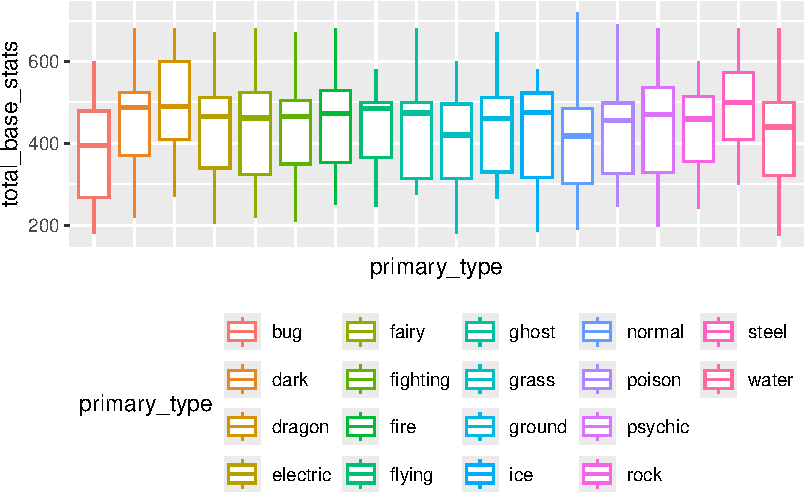
\includegraphics{trabajo_files/figure-pdf/unnamed-chunk-62-1.pdf}

Podemos observar que no hay ningún atípico. Los Pokémon de tipo bicho
(``bug'') son los que tienden a tener una menor suma de estadísticas,
mientras que el acero (``steel'') destaca como uno de los tipos donde la
suma es mayor. Observando las medianas, cerca de estos últimos se
encontrarían los Pokémon de tipo dragón o volador. Parece que las
pequeñas tendencias observadas tienen sentido. Es decir, es razonable
pensar que puede haber cierta relación entre el tipo y las estadísticas.

\begin{figure}[H]

{\centering 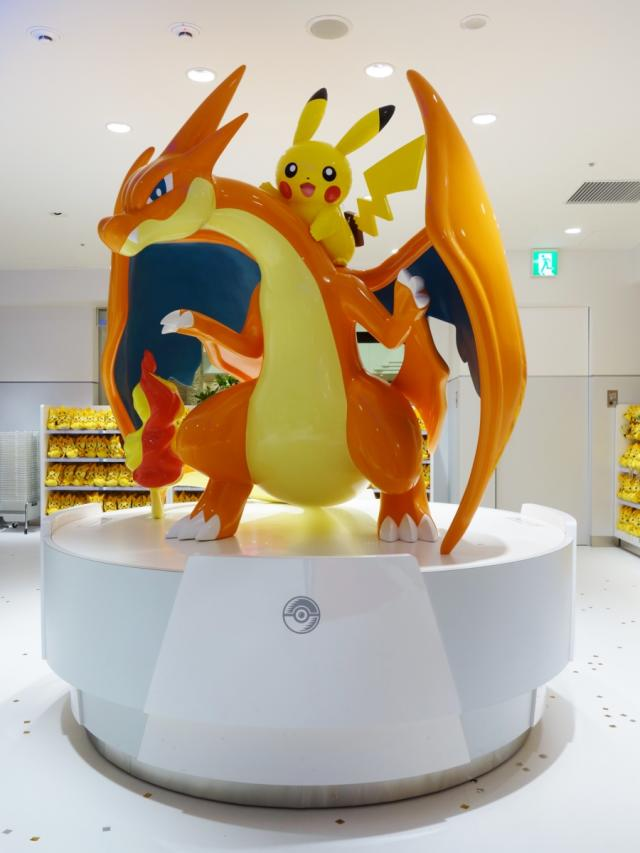
\includegraphics[width=2.39583in,height=\textheight]{trabajo_images/charizard.jpeg}

}

\caption{Figura de Charizard a escala en el Pokémon Center de Tokio
(Japón). Charizard es un Pokémon de primera generación que hemos
obtenido como parte del conjunto de test.}

\end{figure}%

\section{5.2. Entrenamiento del modelo}\label{entrenamiento-del-modelo}

Comenzamos entrenando el modelo con todas las variables de las que
disponemos. Cabe mencionar que, como hemos ``factorizado'' las de
generación y categoría, se introducirán tantas variables \emph{dummy}
como valores (menos uno) tome cada una. Como se trata de regresión
multinomial, hemos de definir una clase de referencia en la variable
respuesta. Parece razonable establecer el tipo ``normal'' como clase de
referencia, dado que podríamos decir que es el ``neutro'' y no está
asociado a ningún elemento ni concepto en específico.

A continuación, entrenamos el modelo. Como hay 18 valores posibles para
el tipo, terminaremos con 17 modelos de regresión logística, cada uno
con 9 variables (predictores) más las que resulten de pasar las
categóricas a dummy. Por tanto, no conviene imprimir el resumen con los
resultados, dado que es tan extenso que no se distingue nada.

Como obtenemos modelos muy complejos, lo más urgente que debemos hacer
ahora es aplicar métodos de selección de regresores, para ver si podemos
reducir la dimensionalidad del modelo y quedarnos solo con los
predictores más relevantes. Vamos a aplicar el método \emph{backward},
con el que hemos obtenido buenos resultados tras algunas pruebas.
También se podrían haber aplicado \emph{forward} o \emph{stepwise}.

Podemos imprimir tras la aplicación del método de selección de
regresores los nombres de las variables con las que ahora opera el
modelo, para las cuales obtenemos coeficientes:

\begin{verbatim}
[1] "(Intercept)"      "total_base_stats" "hp"               "attack"          
[5] "defense"          "special_attack"   "special_defense"  "speed"           
\end{verbatim}

Observamos que nos quedamos únicamente con las variables numéricas, y se
eliminan todas las \emph{dummies} que han surgido de los dos predictores
categóricos. Por tanto, podemos afirmar que las variables
\texttt{generation} y \texttt{category} no tienen especial influencia en
el tipo del Pokémon, como puede ser comprensible (el juego en el que
primero haya aparecido el Pokémon o su categoría no deberían tener
relación con el tipo).

Así, obtenemos como resultado 17 modelos, uno por cada clase que no sea
la de refencia. Cada uno explica el logaritmo de las odds de pertenecer
a un tipo concreto frente a pertenecer al normal. Además, las variables
que influyen en cada uno de estos modelos son las numéricas (``total'',
puntos de salud, ataque, etc.).

\section{5.3. Validación del modelo}\label{validaciuxf3n-del-modelo}

Para este apartado, vamos a obtener predicciones con el modelo
entrenado, tanto en instancias de entrenamiento como de test. Así,
podremos ver su funcionamiento tanto con los datos con los que se ha
construido, como con otros datos desconocidos (pero para los cuales
tenemos sus valores reales del tipo). El objetivo es estudiar si el
modelo ofrece buenas predicciones en general, o si, por el contrario,
subajusta o sobreajusta.




\end{document}
